%   Filename    : chapter_4.tex 
\chapter{Results and Discussion}
This chapter presents the results of the study, specifically TUKIB's various interfaces and pages, features, and backend implementation. As such, the figures shown herein are screenshots of TUKIB.

\section{User Interface}

\subsection{Landing Page}

\figref{fig:landing} showcases the landing page of the website for the system. The page features easy navigation to essential information and pages including home, news and announcements, services, laboratories, and about. A log in button is also included on the top right of the page to ensure that user's can quickly access their accounts. Additionally, a persistent button for the chatbot is found on the bottom left of the page. 

\begin{figure}[h]
	\centering 
	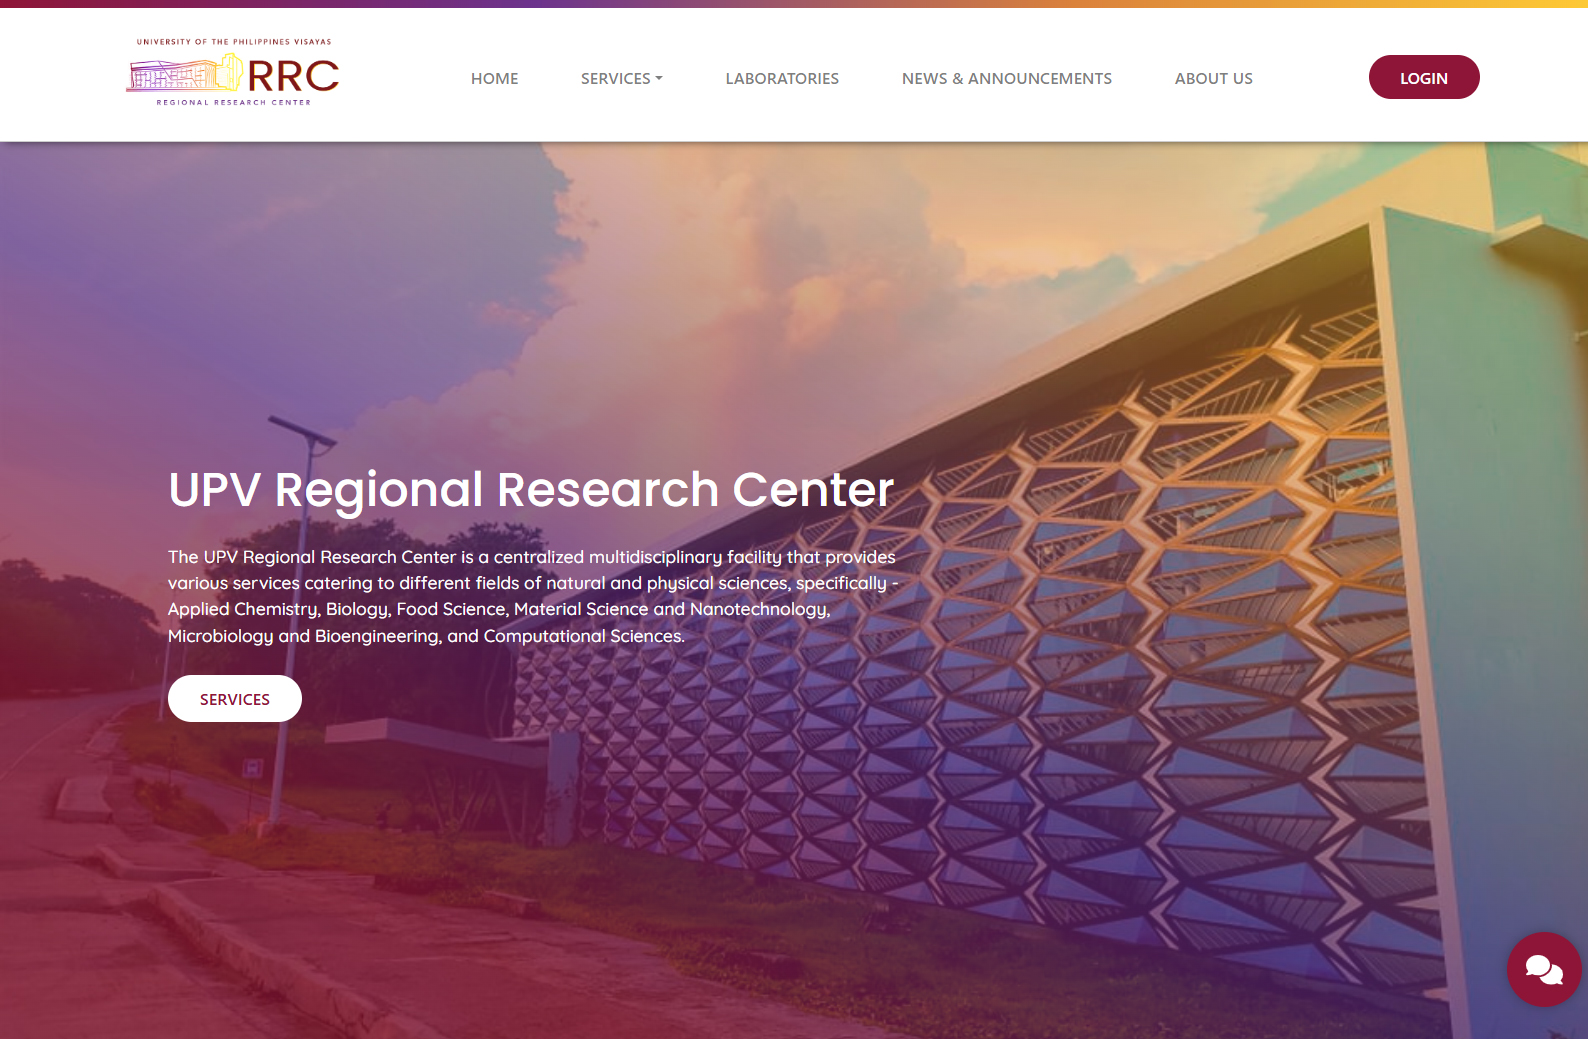
\includegraphics[width=0.75\textwidth]{landing.png}
	\caption{Landing/Homepage}
	\label{fig:landing}
\end{figure}

\subsection{Services Page}

Figure \ref{fig:service_page} shows the `Services' page. Each service has a separate page that includes a description of the service, pricing information, and instructions or guide on how to avail the service. This structure facilitates easier navigation and helps users find the information they need efficiently.

\begin{figure}[h]
	\centering
	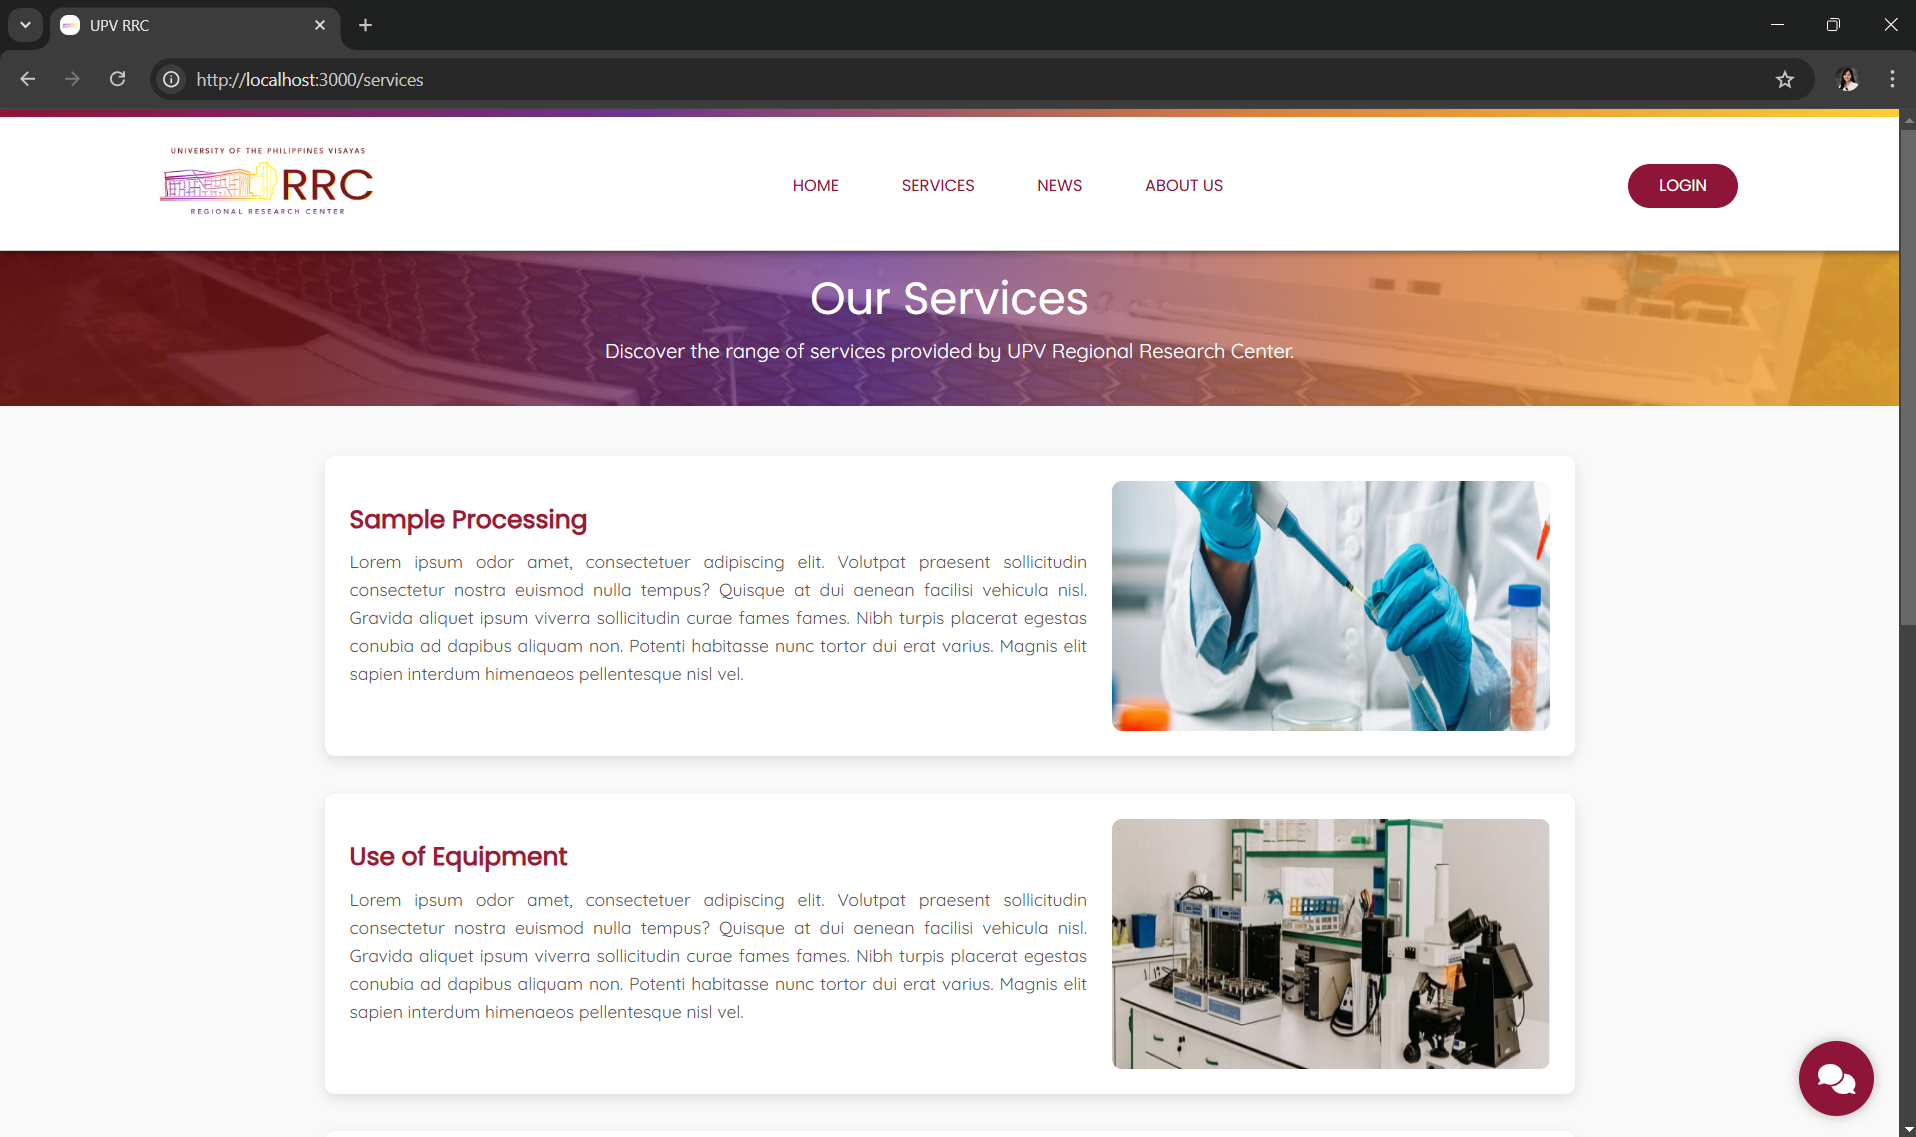
\includegraphics[width=0.75\textwidth]{service_page.png}
	\caption{Services Page}
	\label{fig:service_page}
\end{figure}

\newpage

\subsection{Laboratories Page}

Figure \ref{fig:laboratories_page} shows the `Laboratories' page. This page displays information about the laboratories within the UPV-RRC, including the available equipment and instrument for each lab. It also provides brief descriptions of each piece of equipment to give clients a better understanding of what is available. This helps the clients to make informed decisions when selecting a laboratory for their research needs. 

\begin{figure}[h]
	\centering
	
\includegraphics[width=0.8\textwidth]{laboratories.png}
	\caption{Laboratories Page}
	\label{fig:laboratories_page}
\end{figure}

\newpage

\subsection{News and Announcements Page}

Figure \ref{fig:news_page} is the `News and Announcements' page. This page serves as the central hub for all important updates related to the UPV RRC, including news about upcoming events, recent developments, announcements of new equipment or services, and relevant research highlights.The page contains two tabs, the News tab, and the Announcements tab. The News tab displays the latest news articles, while the Announcements tab contains important notices and updates from the RRC. This structure allows users to easily access and stay informed about the latest happenings at the RRC.

\begin{figure}[h]
	\centering
	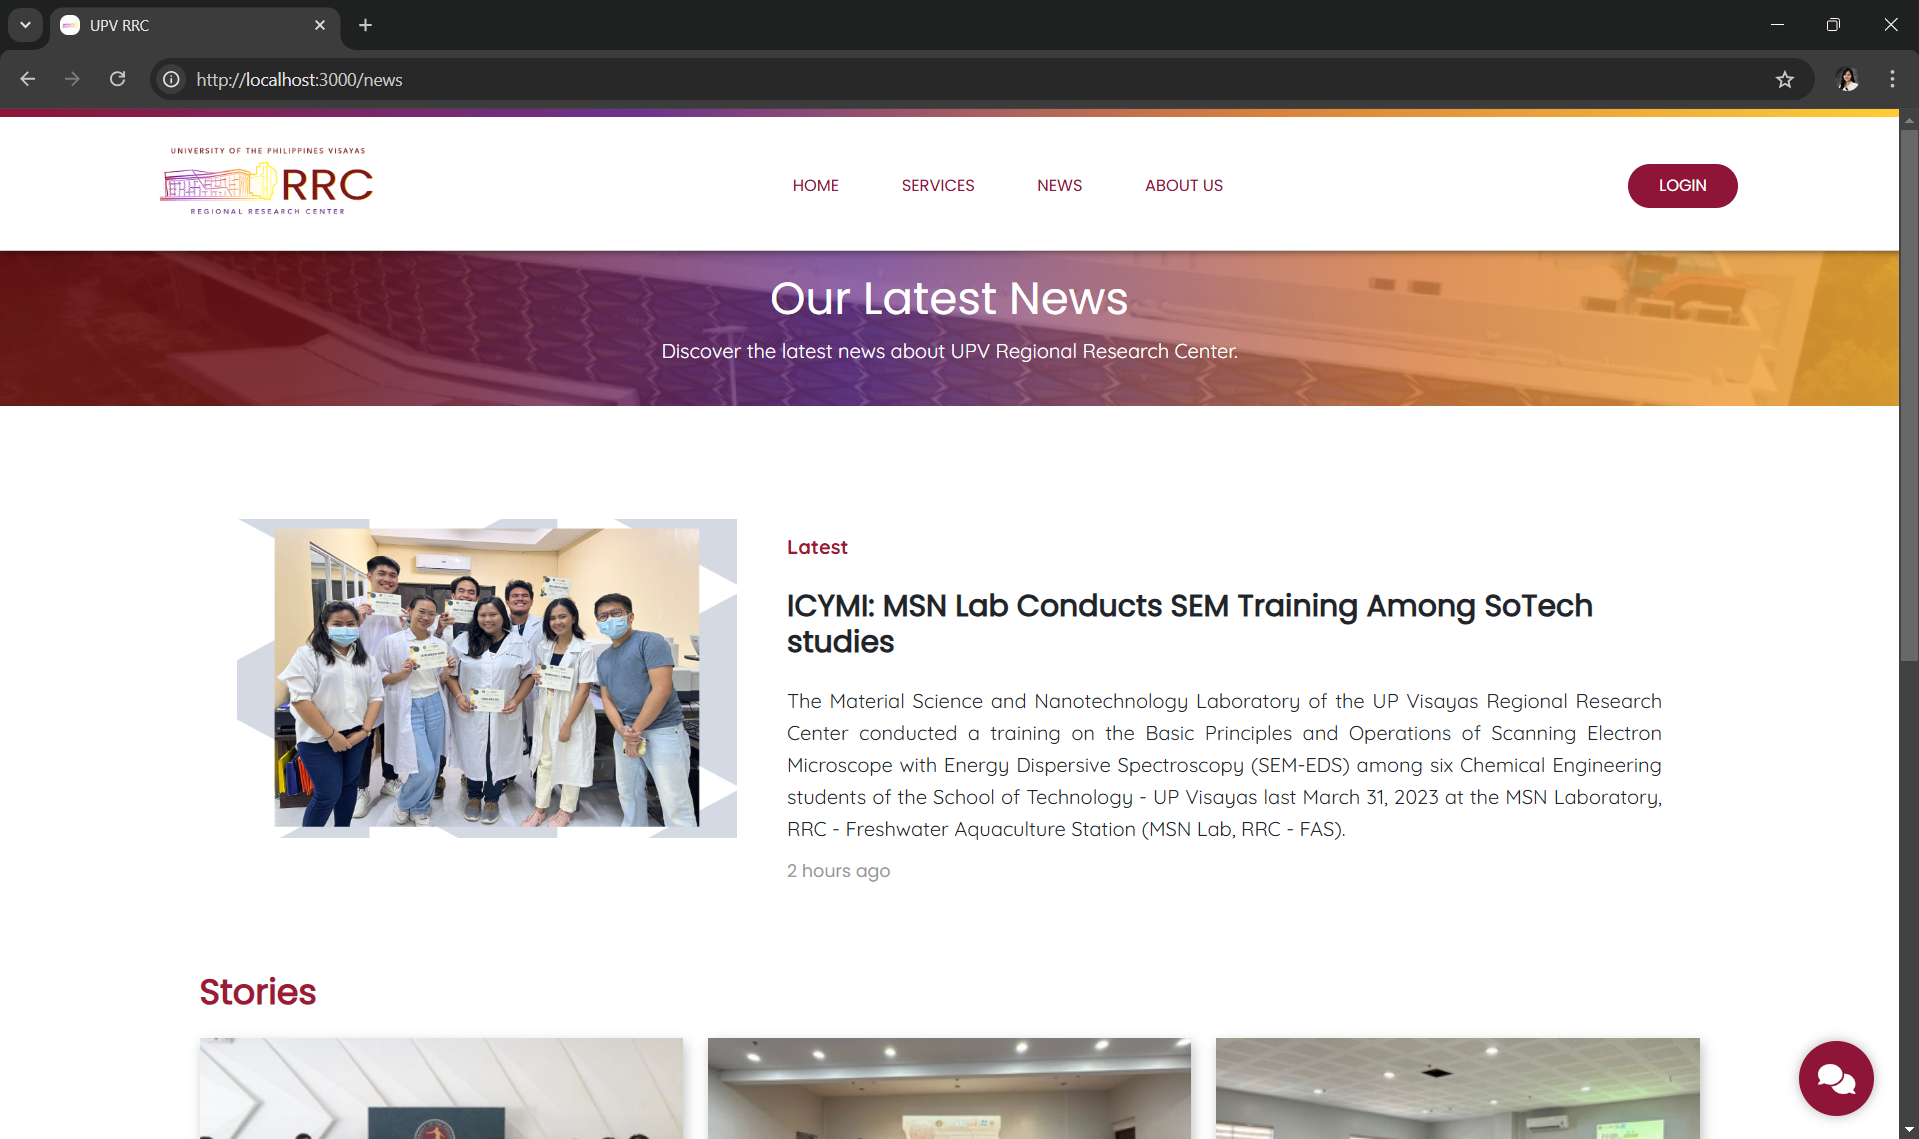
\includegraphics[width=0.7\textwidth]{news_page.png}
	\caption{News Page}
	\label{fig:news_page}
\end{figure}

\newpage

\subsection{About Us Page} 

Figure \ref{fig:about_page} shows the `About Us' page. This page provides an overview of the RRC (Regional Research Center), detailing background information, its mission, vision, and team. It is designed to give visitors a deeper understanding of the organization and its role in the research community.

\begin{figure}[h]
	\centering
	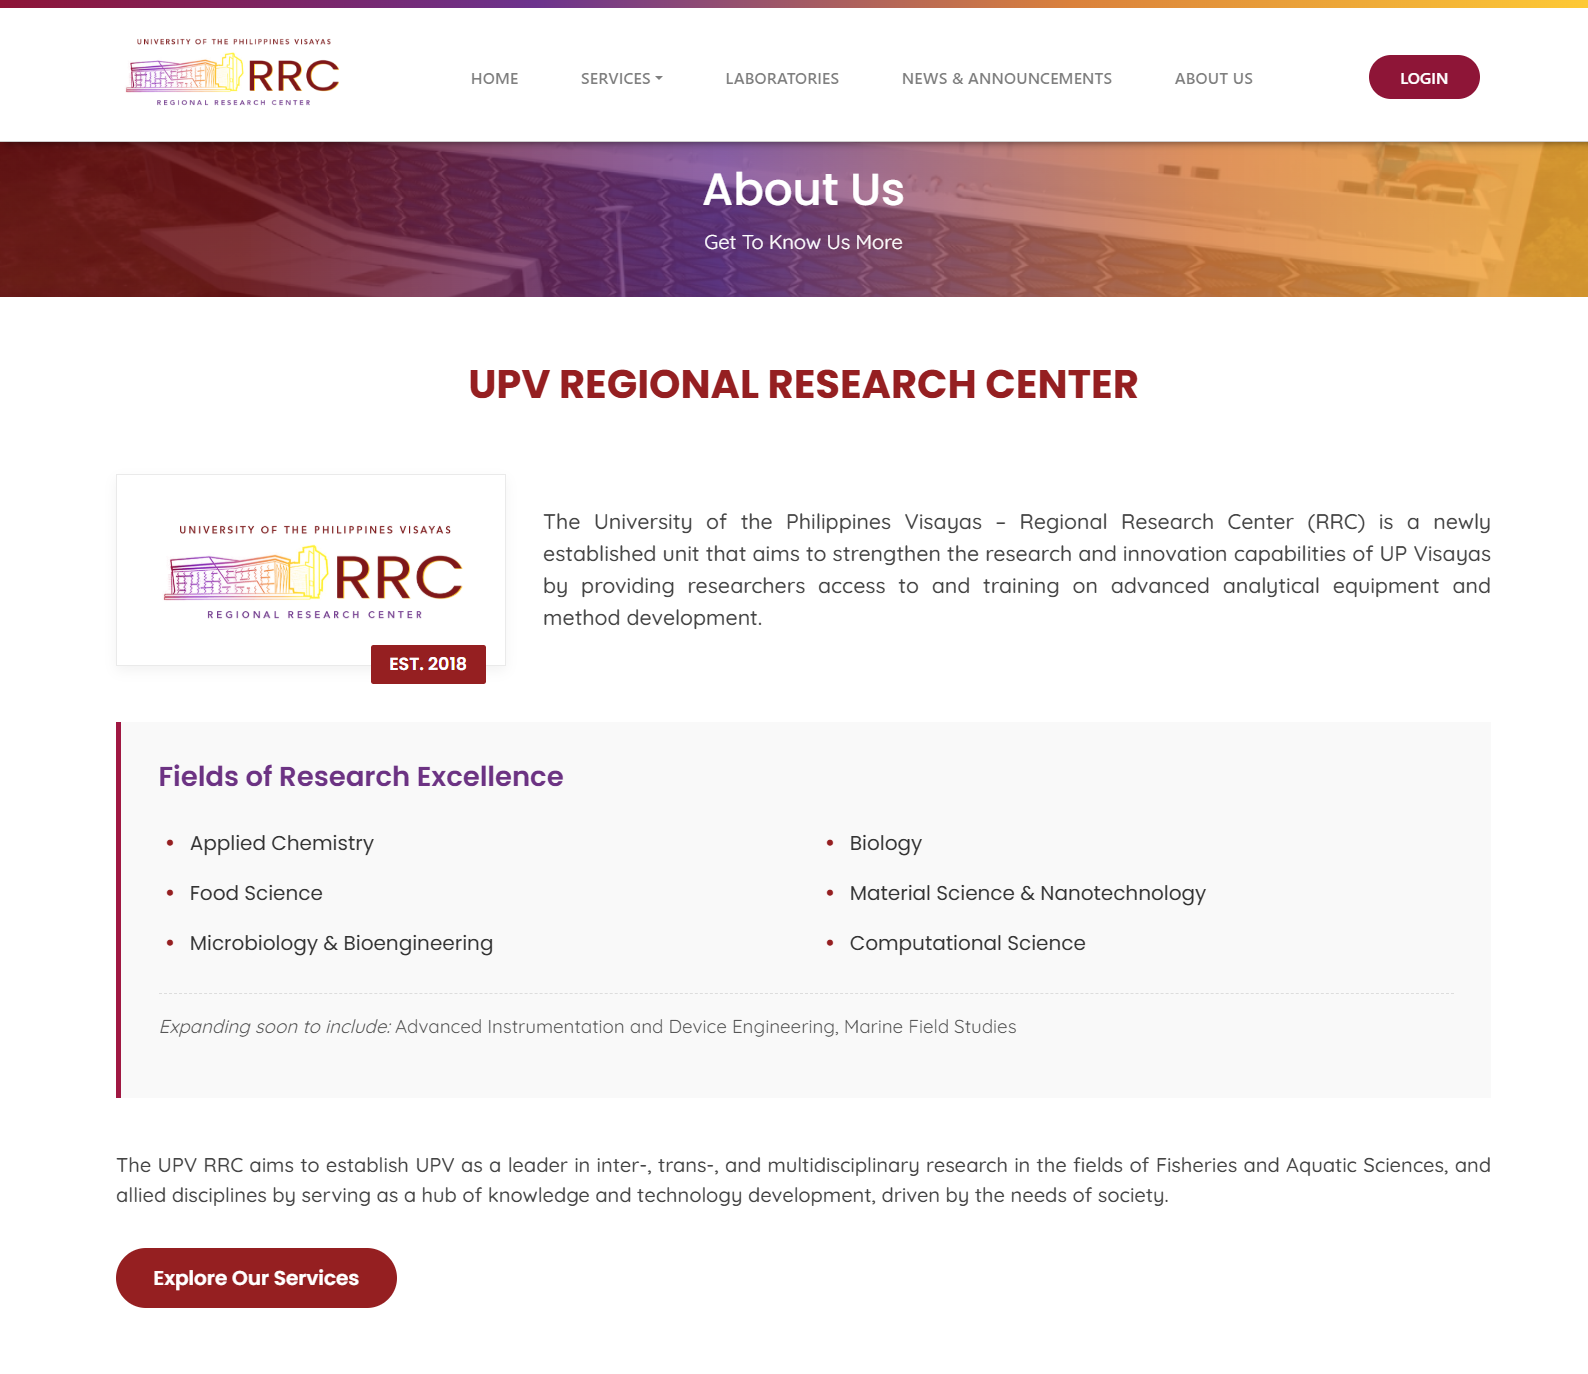
\includegraphics[width=0.8\textwidth]{about_page.png}
	\caption{About Page}
	\label{fig:about_page}
\end{figure}

\subsection{User Dashboards}

User dashboard is designed for the needs of two primary user groups of TUKIB who are the staff and clients. Each user group has a different user interface to cater to their specific needs.

\textbf{Client Dashboard}

The client dashboard is designed with simplicity and usability in mind to support individuals requesting services from the RRC. As shown in \figref{fig:client_dashboard}, the interface provides access to the client's profile, transaction history, and important reminders. A prominent “New Service Request” button is also available, allowing clients to initiate new service requests with ease. This layout ensures clients can efficiently manage their interactions with the RRC while staying informed of their request statuses.

\begin{figure}[h]
	\centering 
	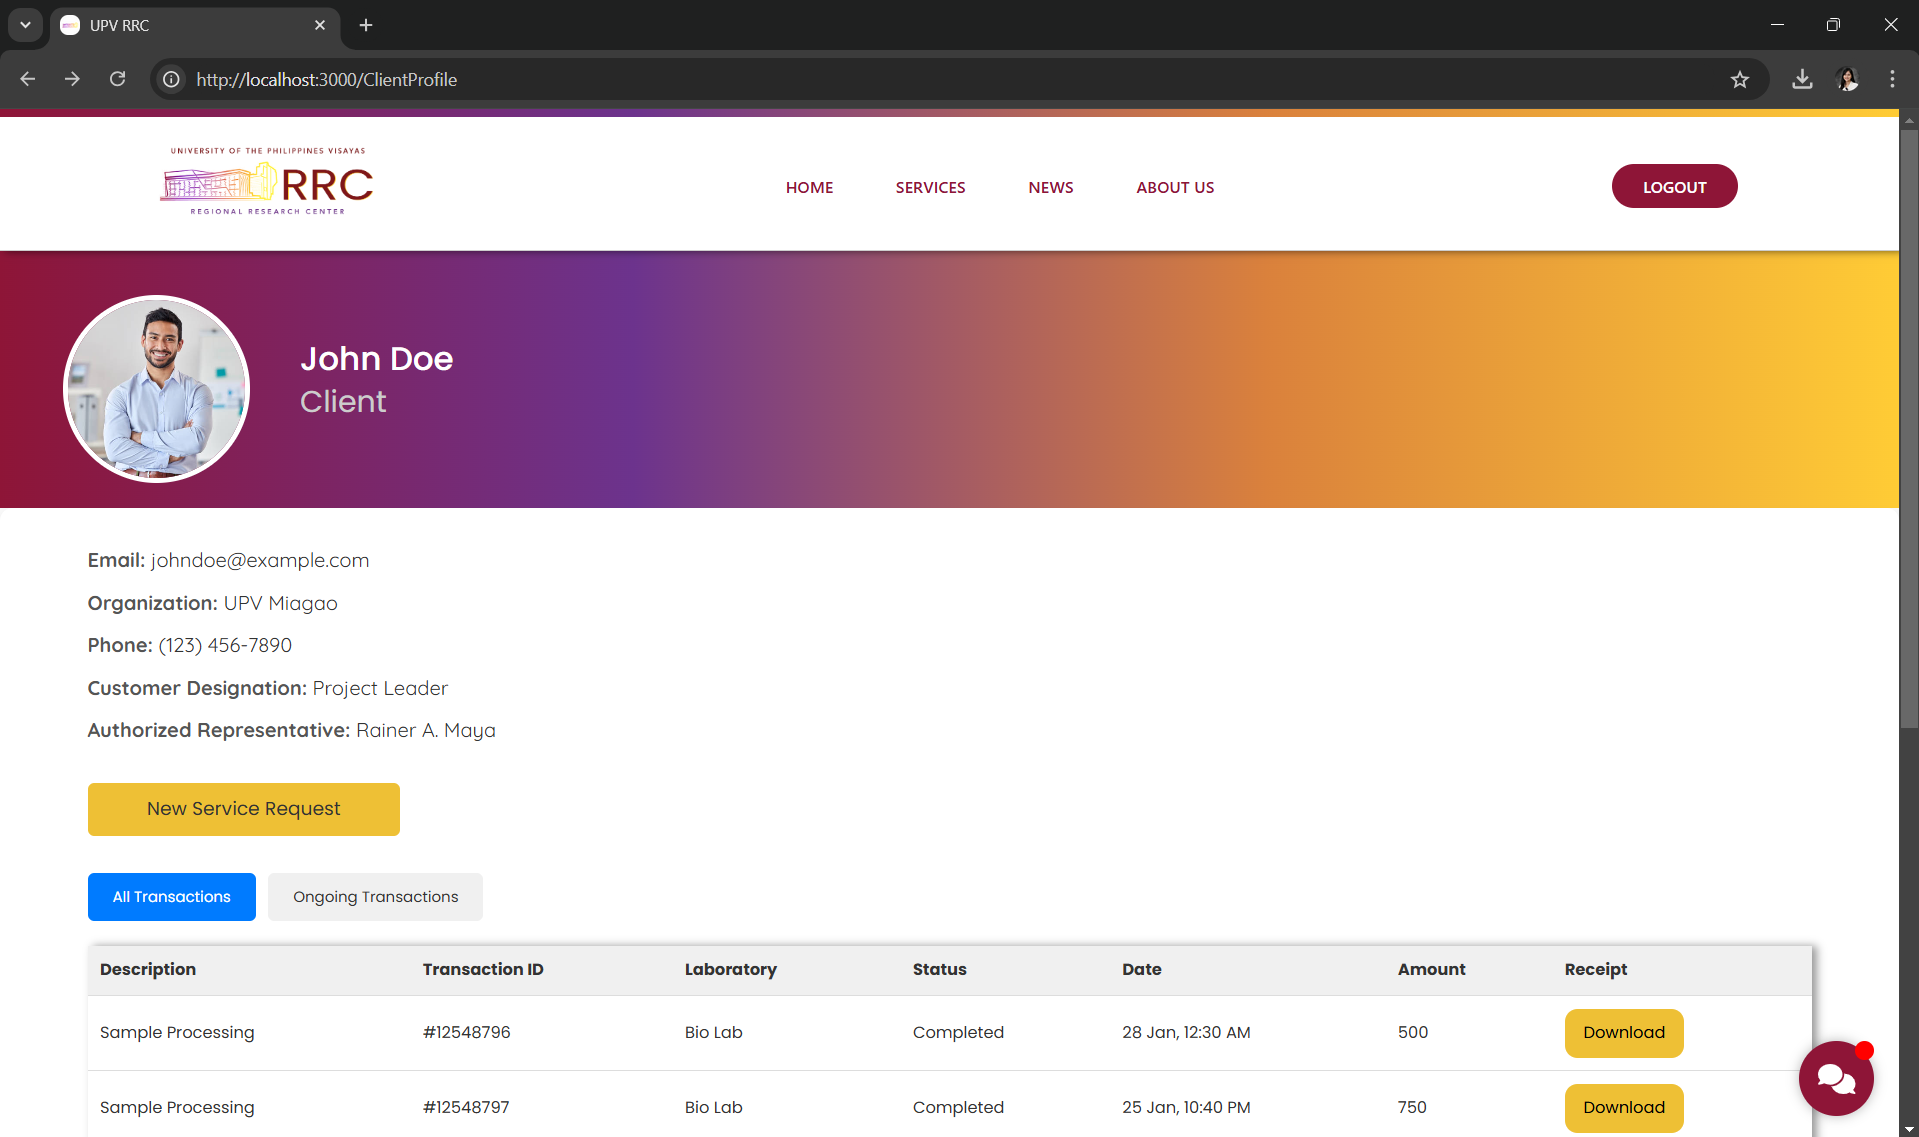
\includegraphics[width=0.8\textwidth]{client_dashboard.png}
	\caption{Client dashboard}
	\label{fig:client_dashboard}
\end{figure}

\newpage

\textbf{Staff Dashboard}

The staff dashboard is designed with role-specific functionalities, depending on the staff member's responsibilities within the RRC. \figref{fig:staff_dashboard} displays the Admin Staff dashboard, which features tabs or sections for managing different aspect of RRC's service workflow. Admin Staff can oversee all client requests, approve or reject service submissions, manage client accounts, manage laboratories, and publish news and announcements.

\begin{figure}[h]
	\centering 
	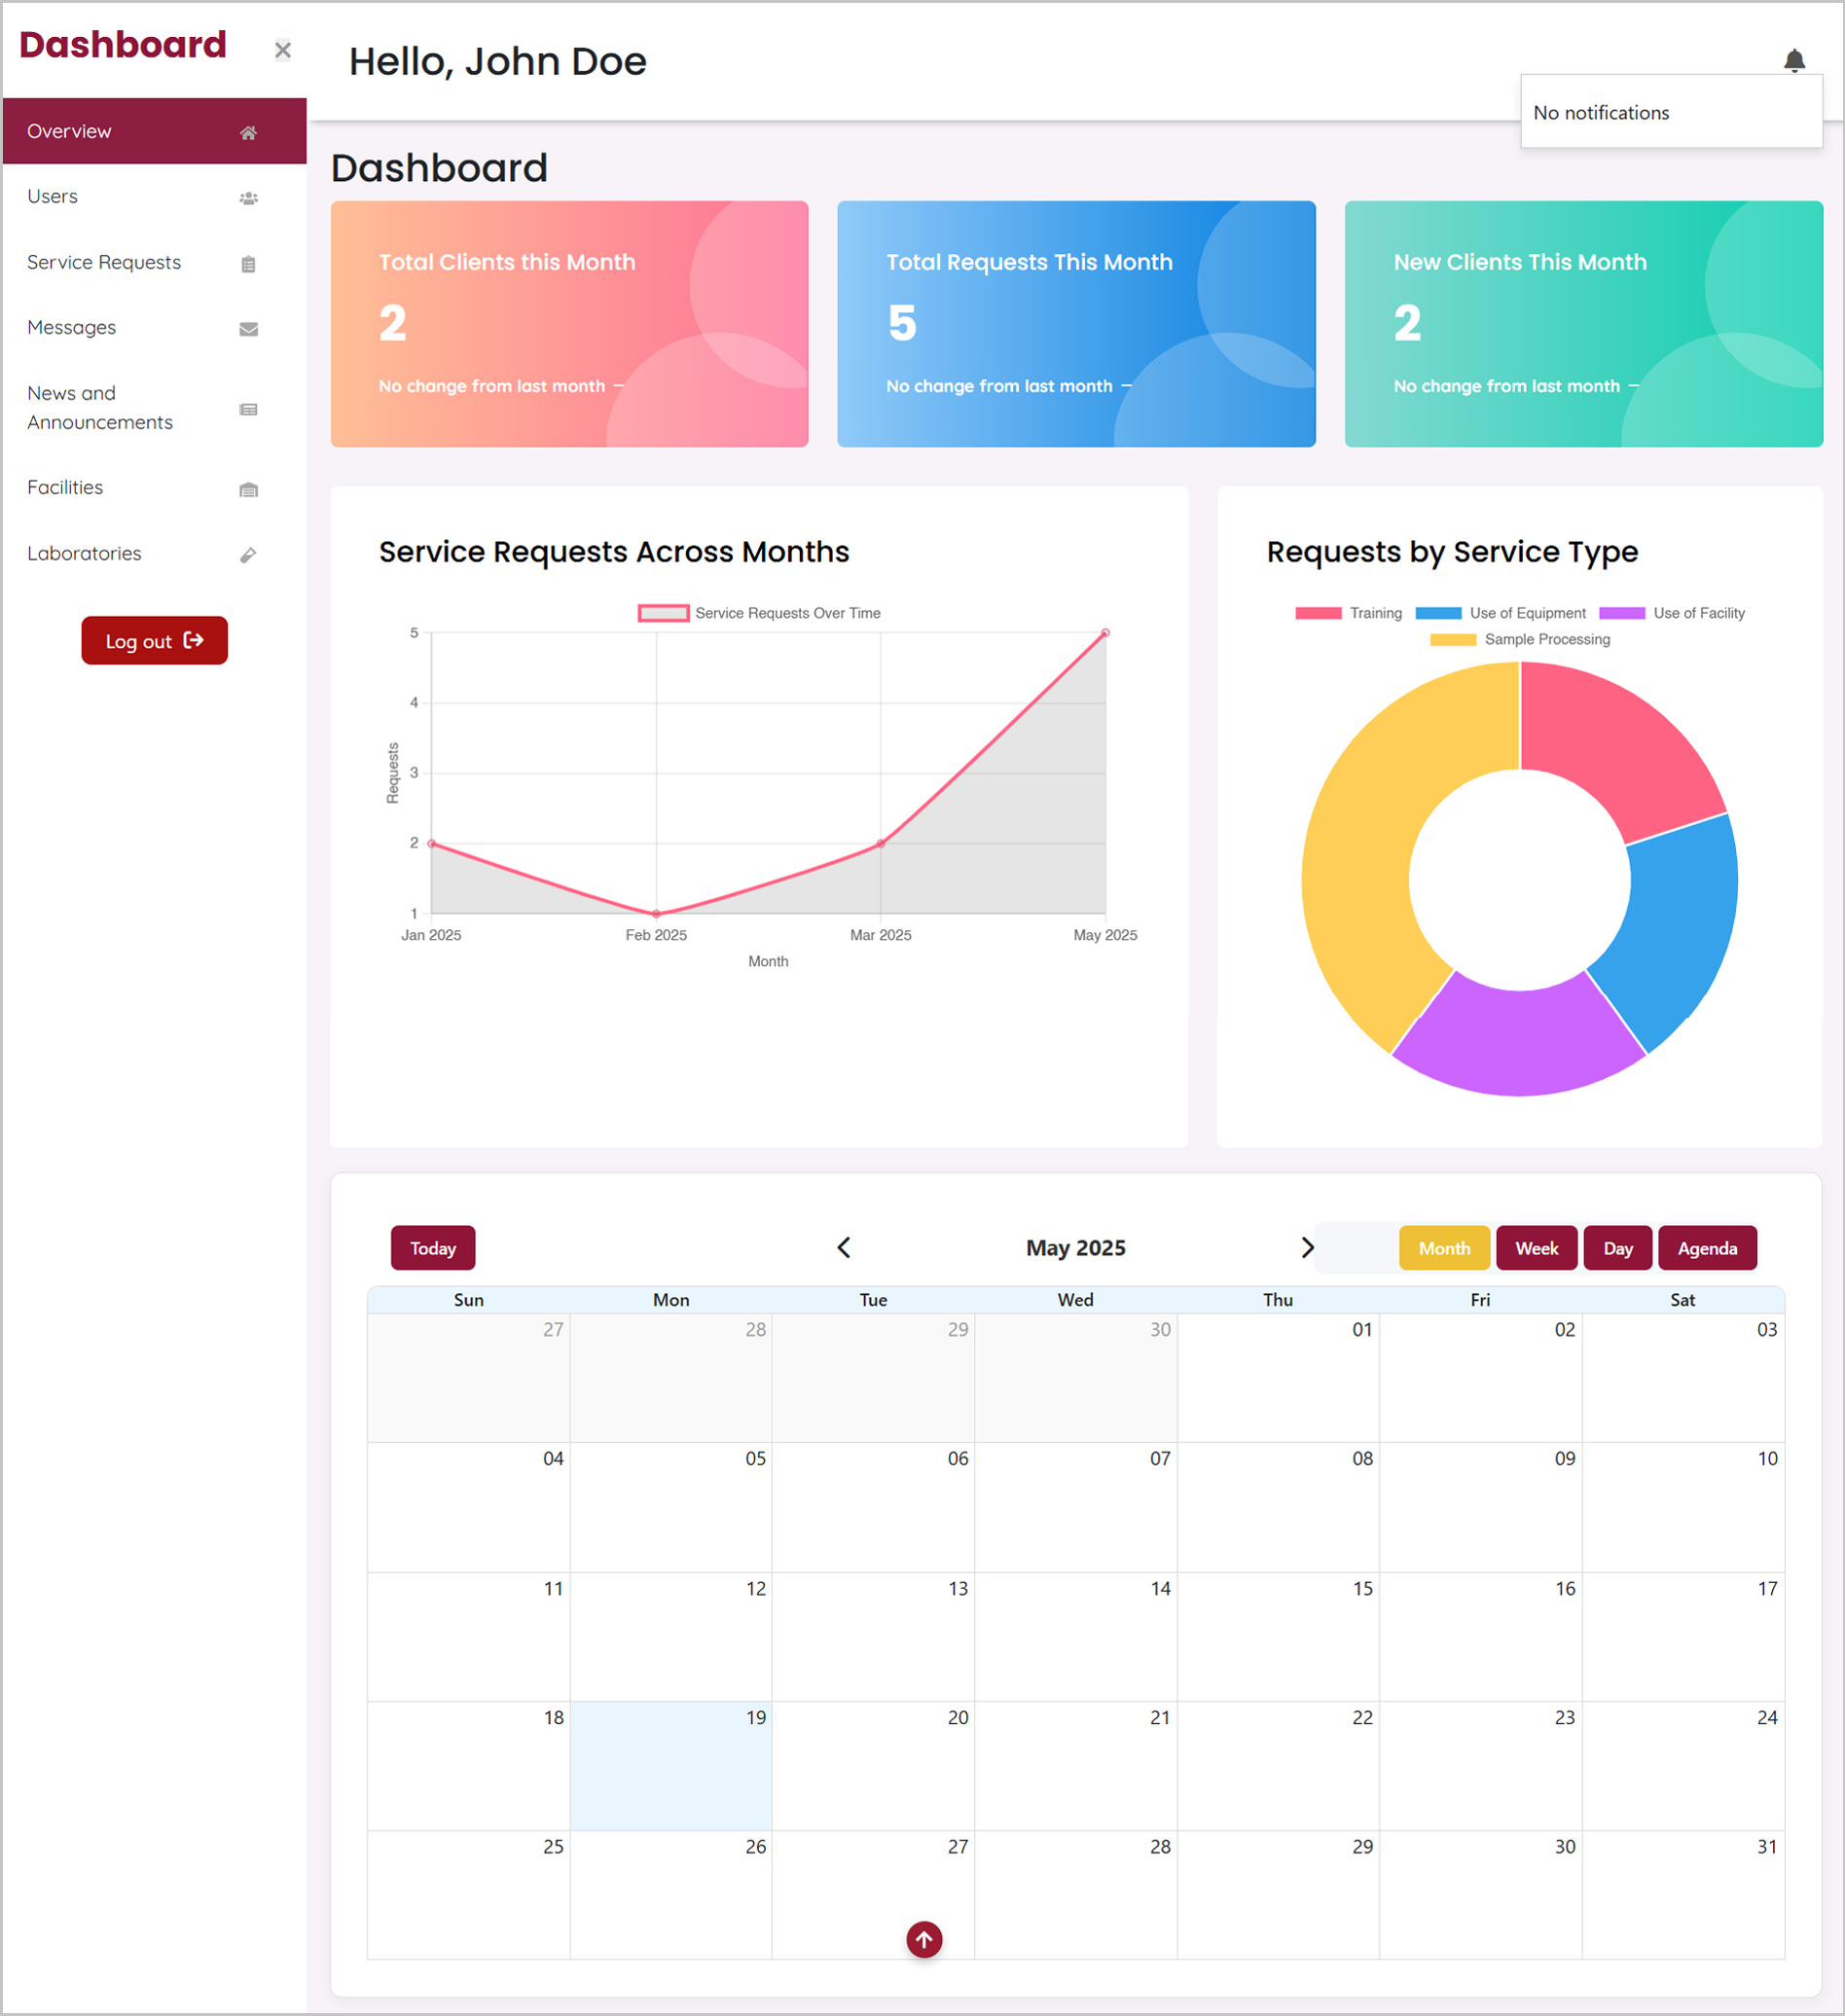
\includegraphics[width=0.8\textwidth]{staff_dashboard.png}
	\caption{Staff dashboard}
	\label{fig:staff_dashboard}
\end{figure}

For other staff members like University Researchers and TECD Staff, their dashboards present tools relevant only to their assigned workflows. This role-based design ensures each staff member can focus on their designated tasks without distractions from unrelated features, improving efficiency and clarity.

\section{System Features}

\subsection{User Management Module}

\textbf{User registration}

Clients can create their own accounts through the sign in page. However, by default, these accounts will remain inactive until the Admin Staff approves them after reviewing their information. An additional step is required in which they must undergo an initial consultation with the staff. Only after this consultation will their account be permitted to submit a service request. This process ensures that new clients are informed about the proper procedures for requesting a service, as consultation is a necessary step.

As shown in \figref{fig:signup_page}, the sign-up page collects essential information such as the client's full name, email (used to notify them when their account is approved and becomes active), contact number, institution, and a password. This ensures that the system gathers all relevant details needed for account verification and further communication. Proper input validation mechanisms are also in place to ensure data integrity—for example, email addresses must be unique to prevent duplicate accounts, and all required fields must be properly filled before submission.

On the other hand, staff accounts are pre-made by the Admin Staff. This approach ensures that only authorized personnel are granted access to the system’s internal functions, promoting security and controlled user management.

\begin{figure}[h]
	\centering 
	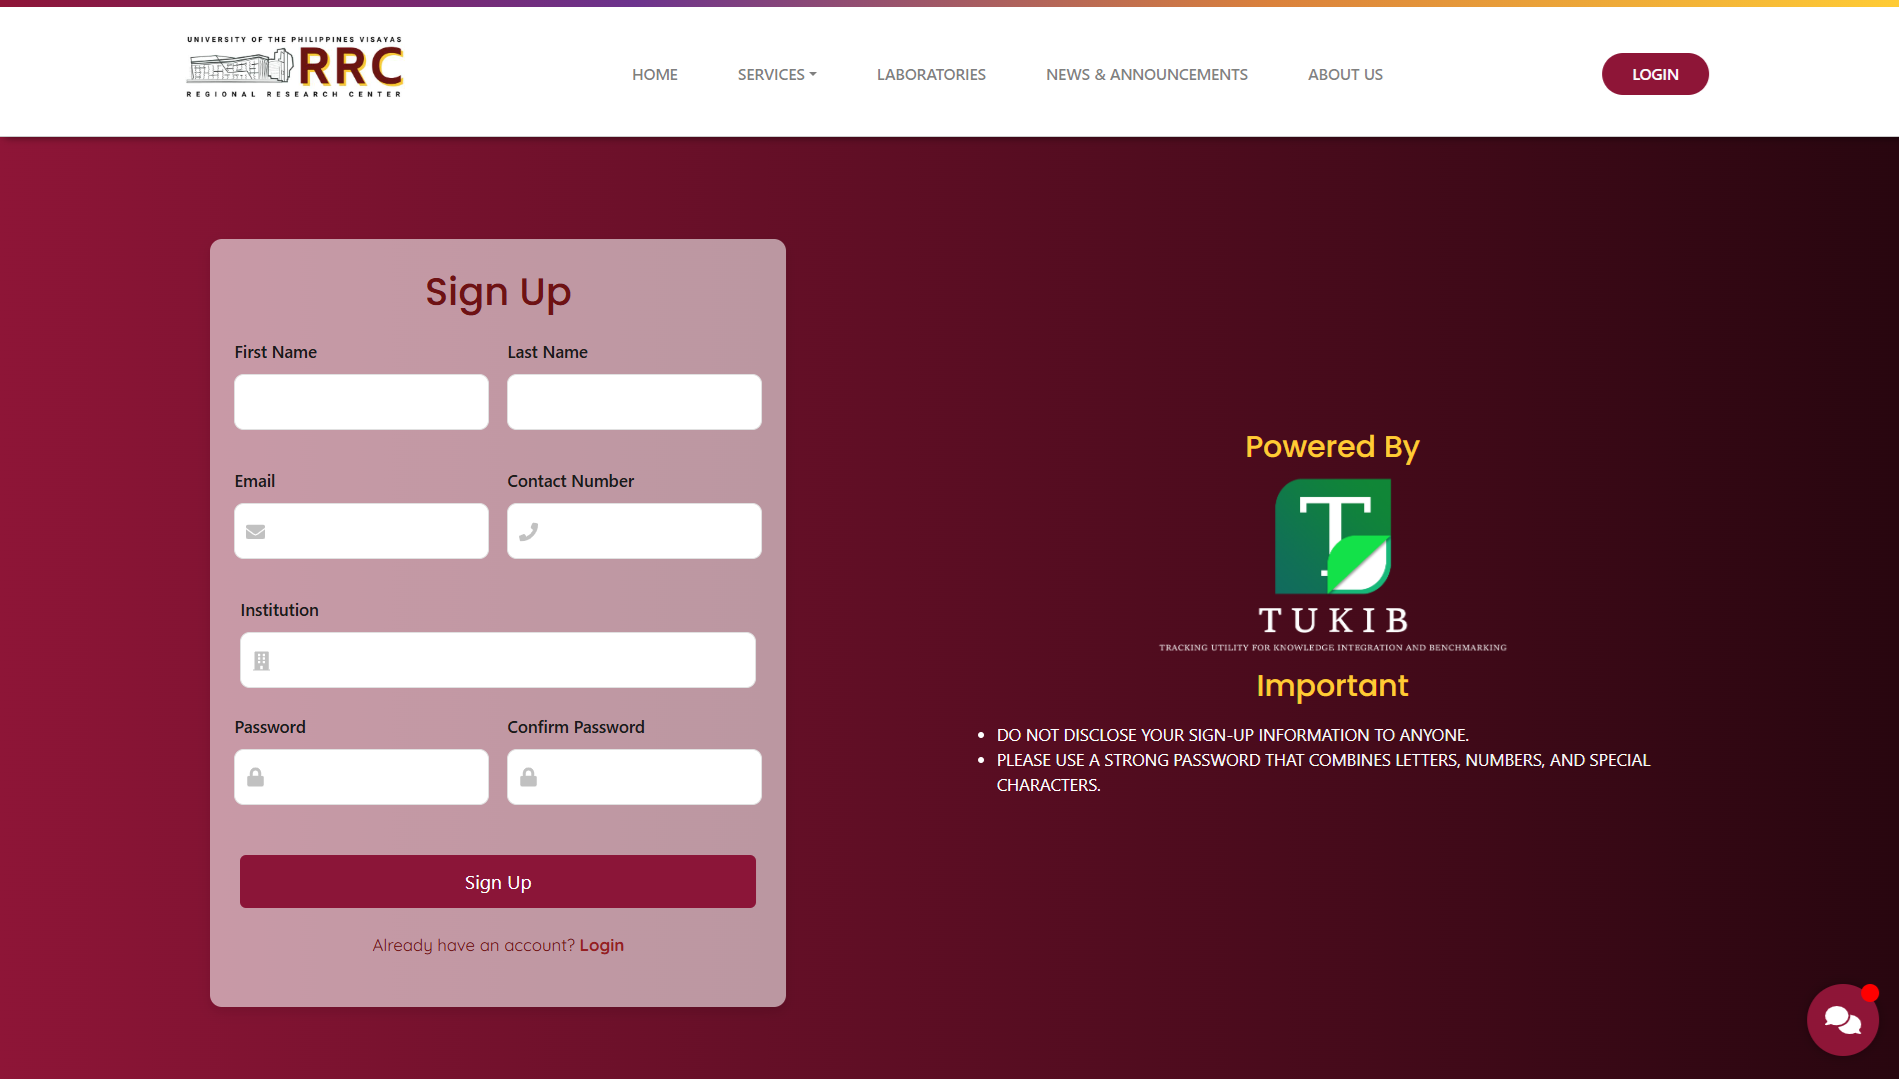
\includegraphics[width=0.8\textwidth]{sign_up.png}
	\caption{Sign Up Page}
	\label{fig:signup_page}
\end{figure}

\textbf{User authentication}

On the login page, users need to enter their email address and password. Additionally, Google authentication is available, allowing users to sign in using their Google account for a quicker and more secure login experience. Passwords are hidden by default, but users can click the eye icon in the password field (as shown in \figref{fig:login}) to toggle visibility. After successfully logging in, users will be redirected to their respective dashboards.

\begin{figure}[h]
	\centering 
	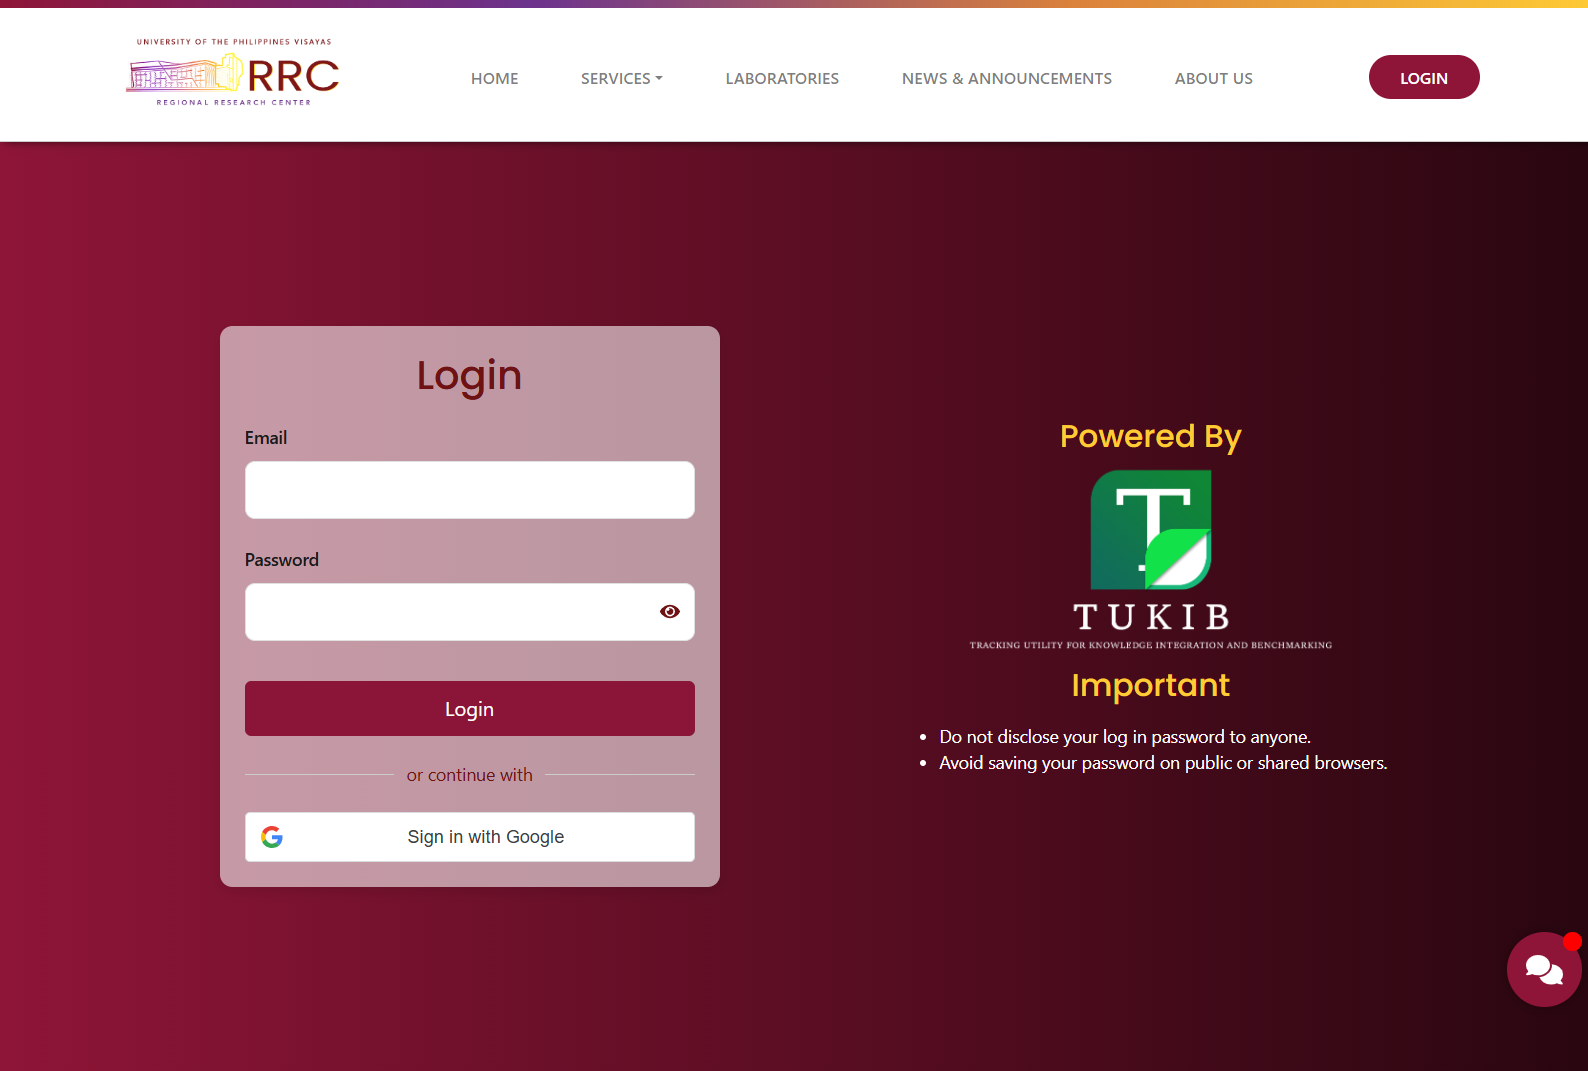
\includegraphics[width=0.8\textwidth]{login.png}
	\caption{Log In Page}
	\label{fig:login}
\end{figure}

\subsection{Service Request Module}

One of the core features of TUKIB is the Service Request Module, which enables both clients and staff to efficiently access, track, and manage service requests through their respective accounts. Clients can submit service requests, monitor the status of their requests, upload payment receipts, view results, and provide feedback to the UPV Regional Research Center. On the other hand, staff members have the capability to approve or reject requests, update request statuses, upload charge slips and results, and review payment receipts submitted by clients. This bidirectional functionality ensures that each request is processed smoothly from initiation to completion.

\figref{fig:service_request_details} displays the full service request details page. This page contains comprehensive information about a specific request and is accessible to both clients and staff, depending on their role. It includes key details such as the type of service requested, current status, payment information, and required documents. A progress indicator is also provided to help both parties track the current stage of the request.

Additionally, role-based functionalities are implemented to tailor the interface to each user's responsibilities. For instance, staff users can approve requests, generate charge slips, and upload final results. Meanwhile, clients can upload payment receipts, view results, and provide feedback.

\begin{figure}[h]
	\centering 
	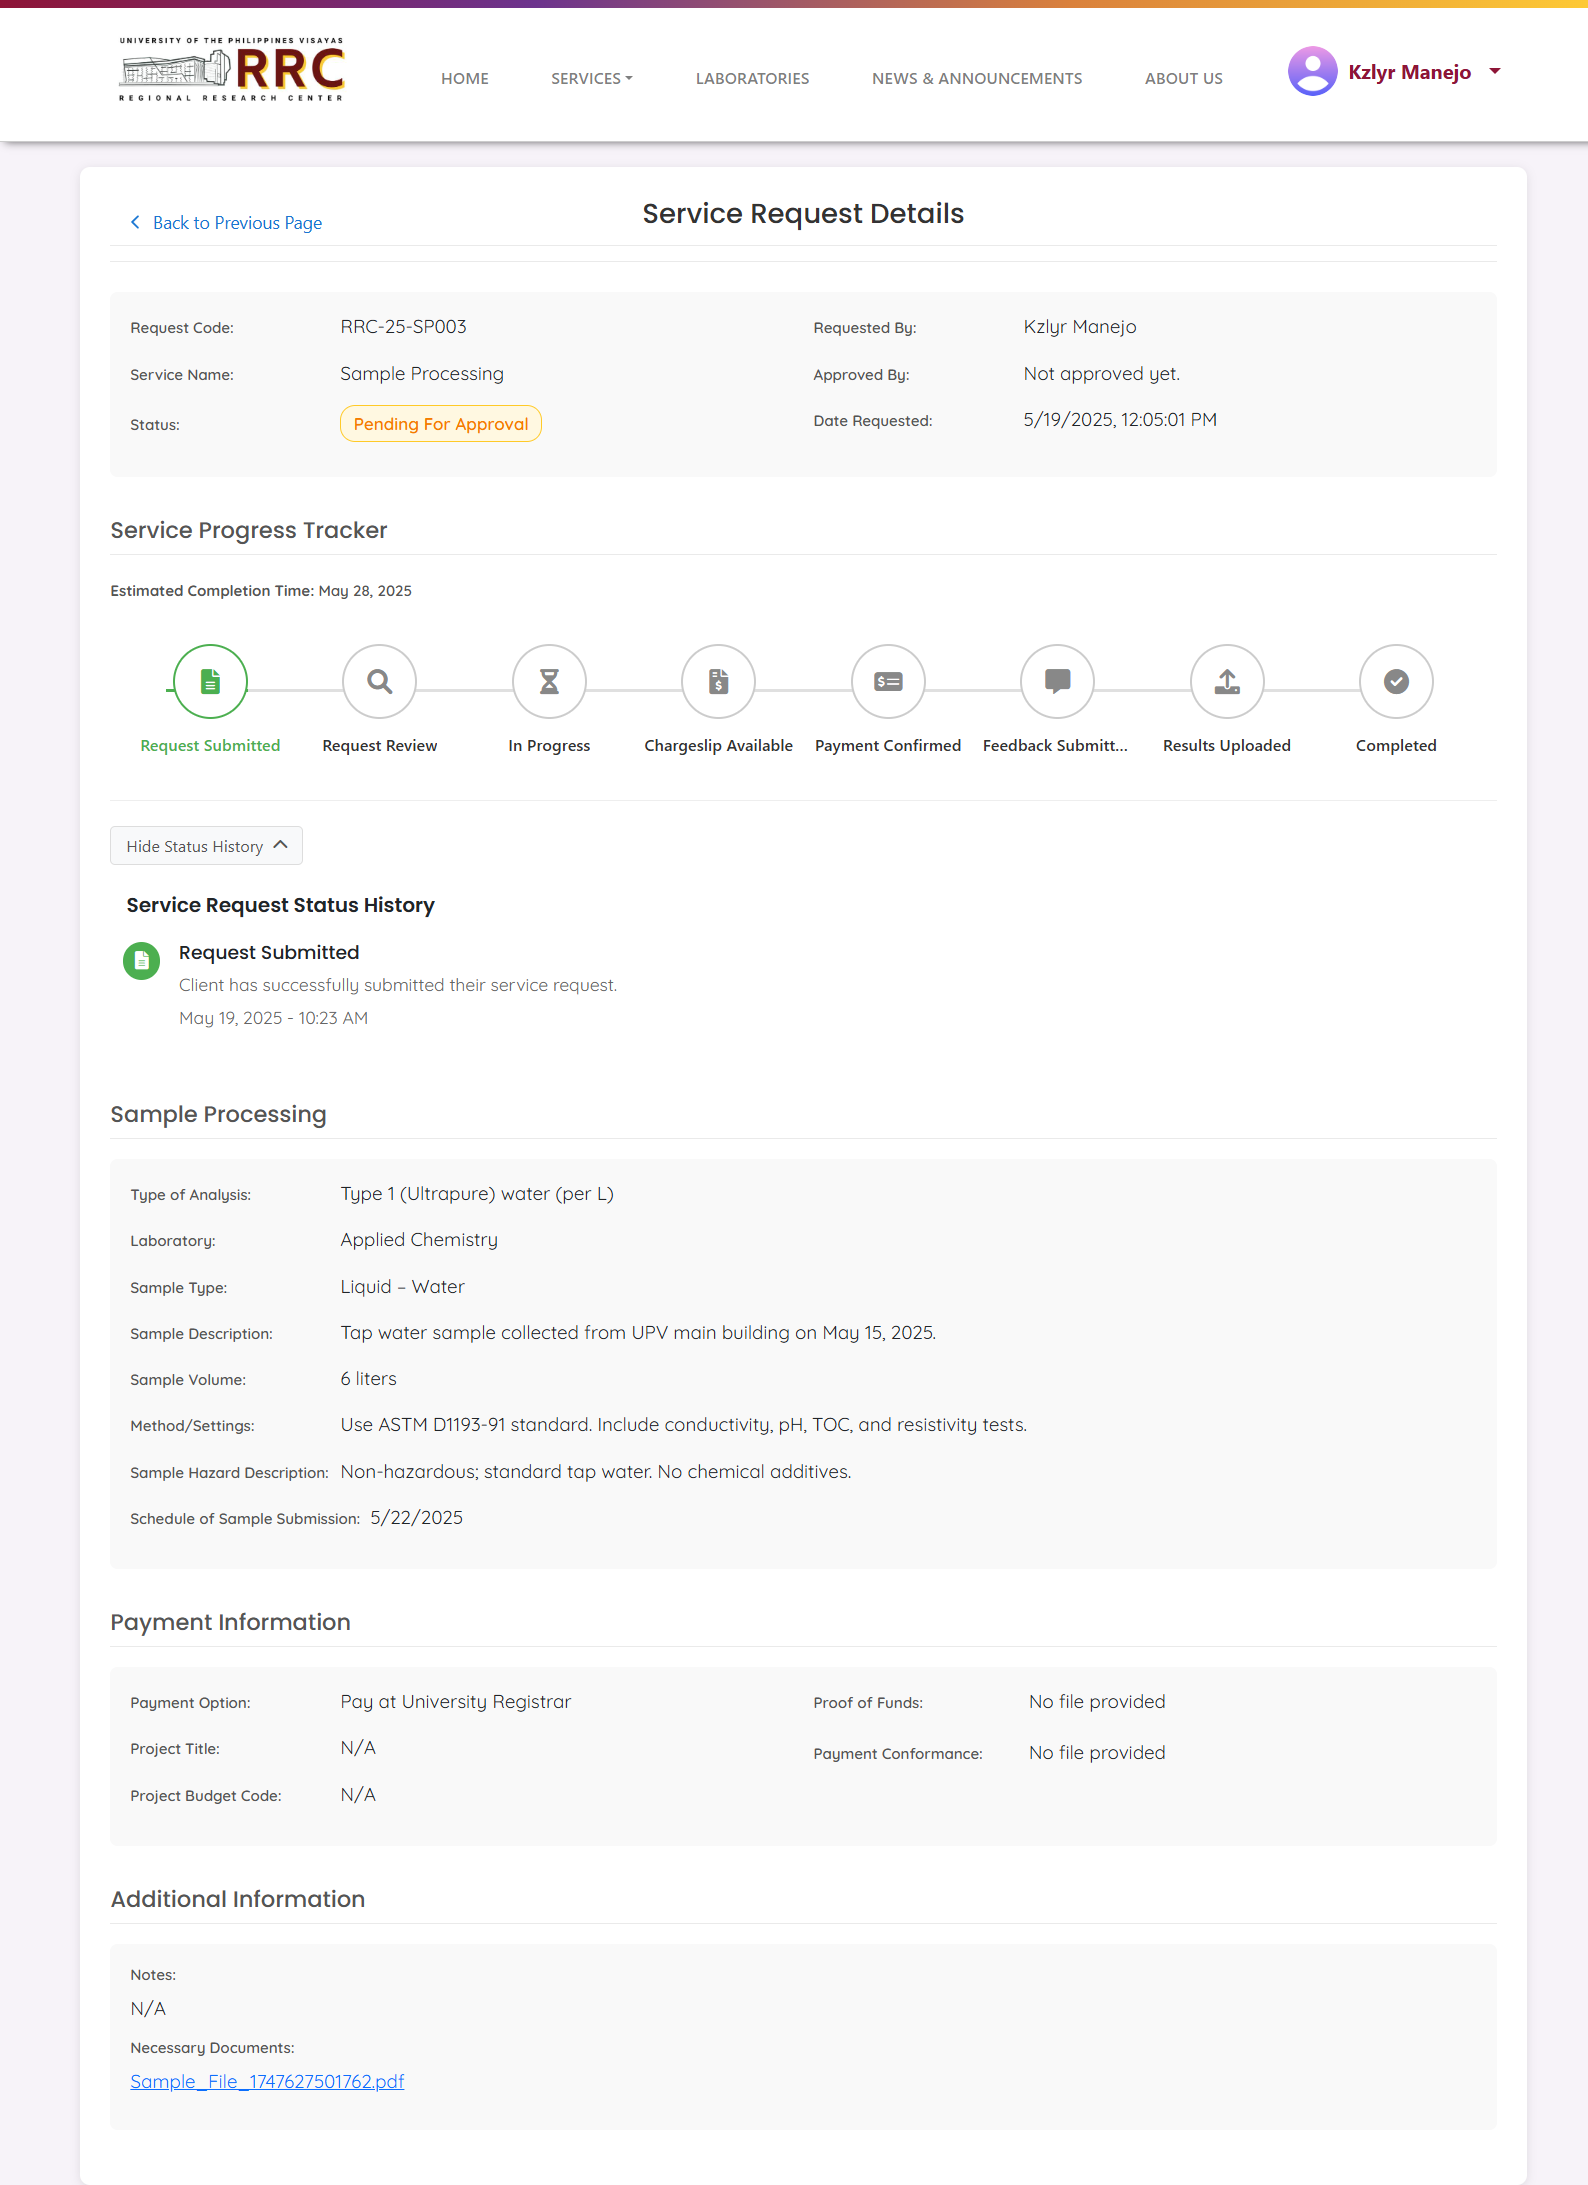
\includegraphics[width=0.75\textwidth]{service_request_details.png}
	\caption{Service Request Details Page}
	\label{fig:service_request_details}
\end{figure}

\newpage

\subsection{Calendar and Scheduling Module}

To effectively manage service schedules, TUKIB includes a Calendar and Scheduling Module. This enables staff to view and track scheduled services in a clear and organized format. There are four types of calendars within the system: general, laboratory, equipment, and facility.

The general calendar serves as an overview of all the institution's activities. When a date is marked as unavailable or restricted in the system calendar— may it be due to holidays, maintenance, or other events—it is automatically blocked across all laboratory, equipment, and facility calendars, preventing any requests from client for that date. This calendar is managed by the Admin Staff and Director.

The calendar for laboratory is designed for managing schedules specific to each laboratory. Every laboratory has its own dedicated calendar displaying unavailable dates and available date and time slots. University Researchers overseeing a laboratory can optionally choose to include some or all equipment, within the laboratory, under the same scheduling restrictions when managing service availability.

In addition, each piece of equipment has its own calendar to track availability. This helps prevent double bookings. Similarly, each Facility, such as conference rooms or audio/visual rooms, has its own calendar to manage usage and avoid scheduling conflicts.

All calendars are interactive and updated in real time. Changes such as request approvals, rejections, or cancellations are reflected immediately, allowing users and staff to make informed decisions and avoid scheduling conflicts.

The calendar is interactive and updated in real time, ensuring that any unavailability or availability is communicated across staff and clients. This module enhances transparency, supports better planning, and contributes to a smoother service flow within TUKIB.

Figure~\ref{fig:calendar} shows the calendar interface within the system. When a date is clicked, a form will be shown asking for necessary details regarding its unavailability of the date.

\begin{figure}[h]
    \centering
    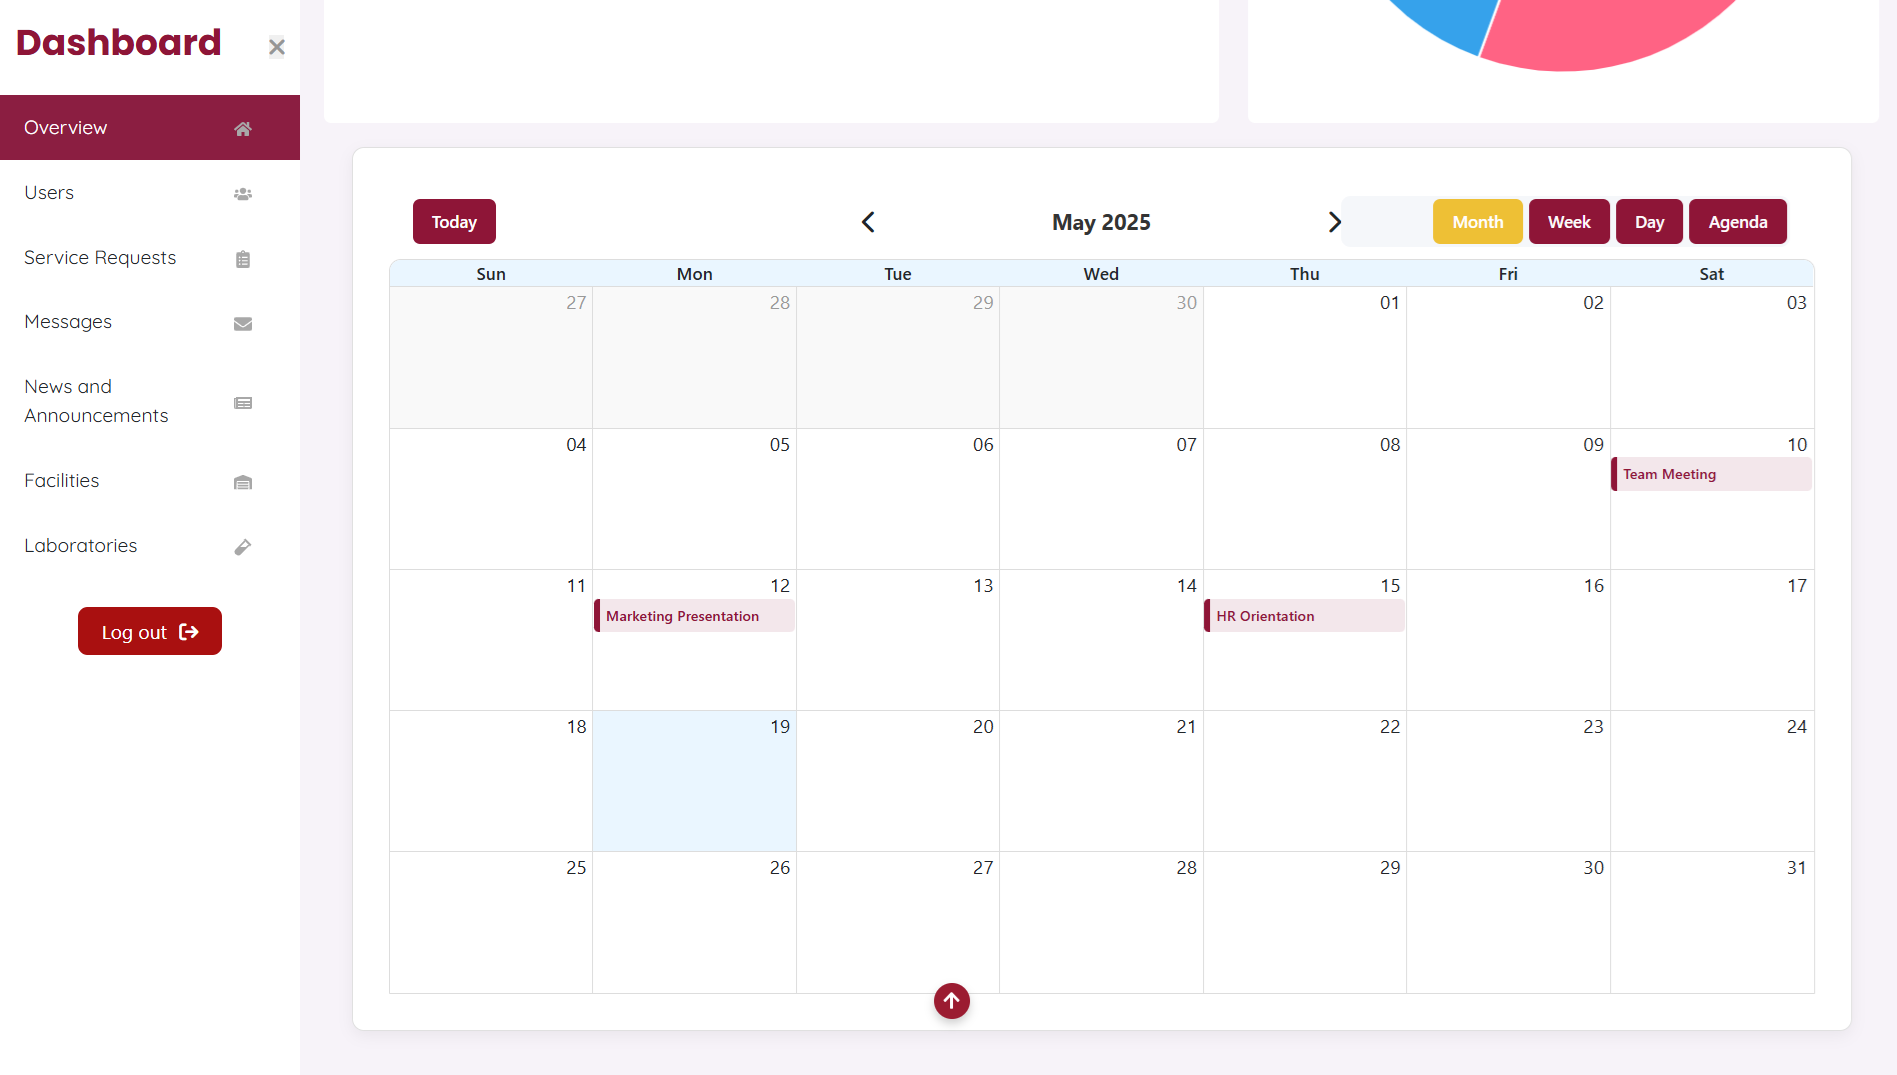
\includegraphics[width=0.8\textwidth]{calendar.png}
    \caption{Calendar}
    \label{fig:calendar}
\end{figure}

\newpage

\subsection{News and Announcement Module}

To facilitate efficient communication between the RRC and its stakeholders, the system features a News and Announcement Module. This allows Admin Staff and TECD Staff to create and post important public updates, news, and announcements directly within the platform, particularly those related to the RRC and its services.

As seen in \figref{fig:announcements}, the module provides fields for entering a title, composing the content, and uploading relevant images. This ensures that relevant information such as upcoming RRC events, service changes, and newly available equipment is effectively communicated.

\begin{figure}[h]
    \centering
    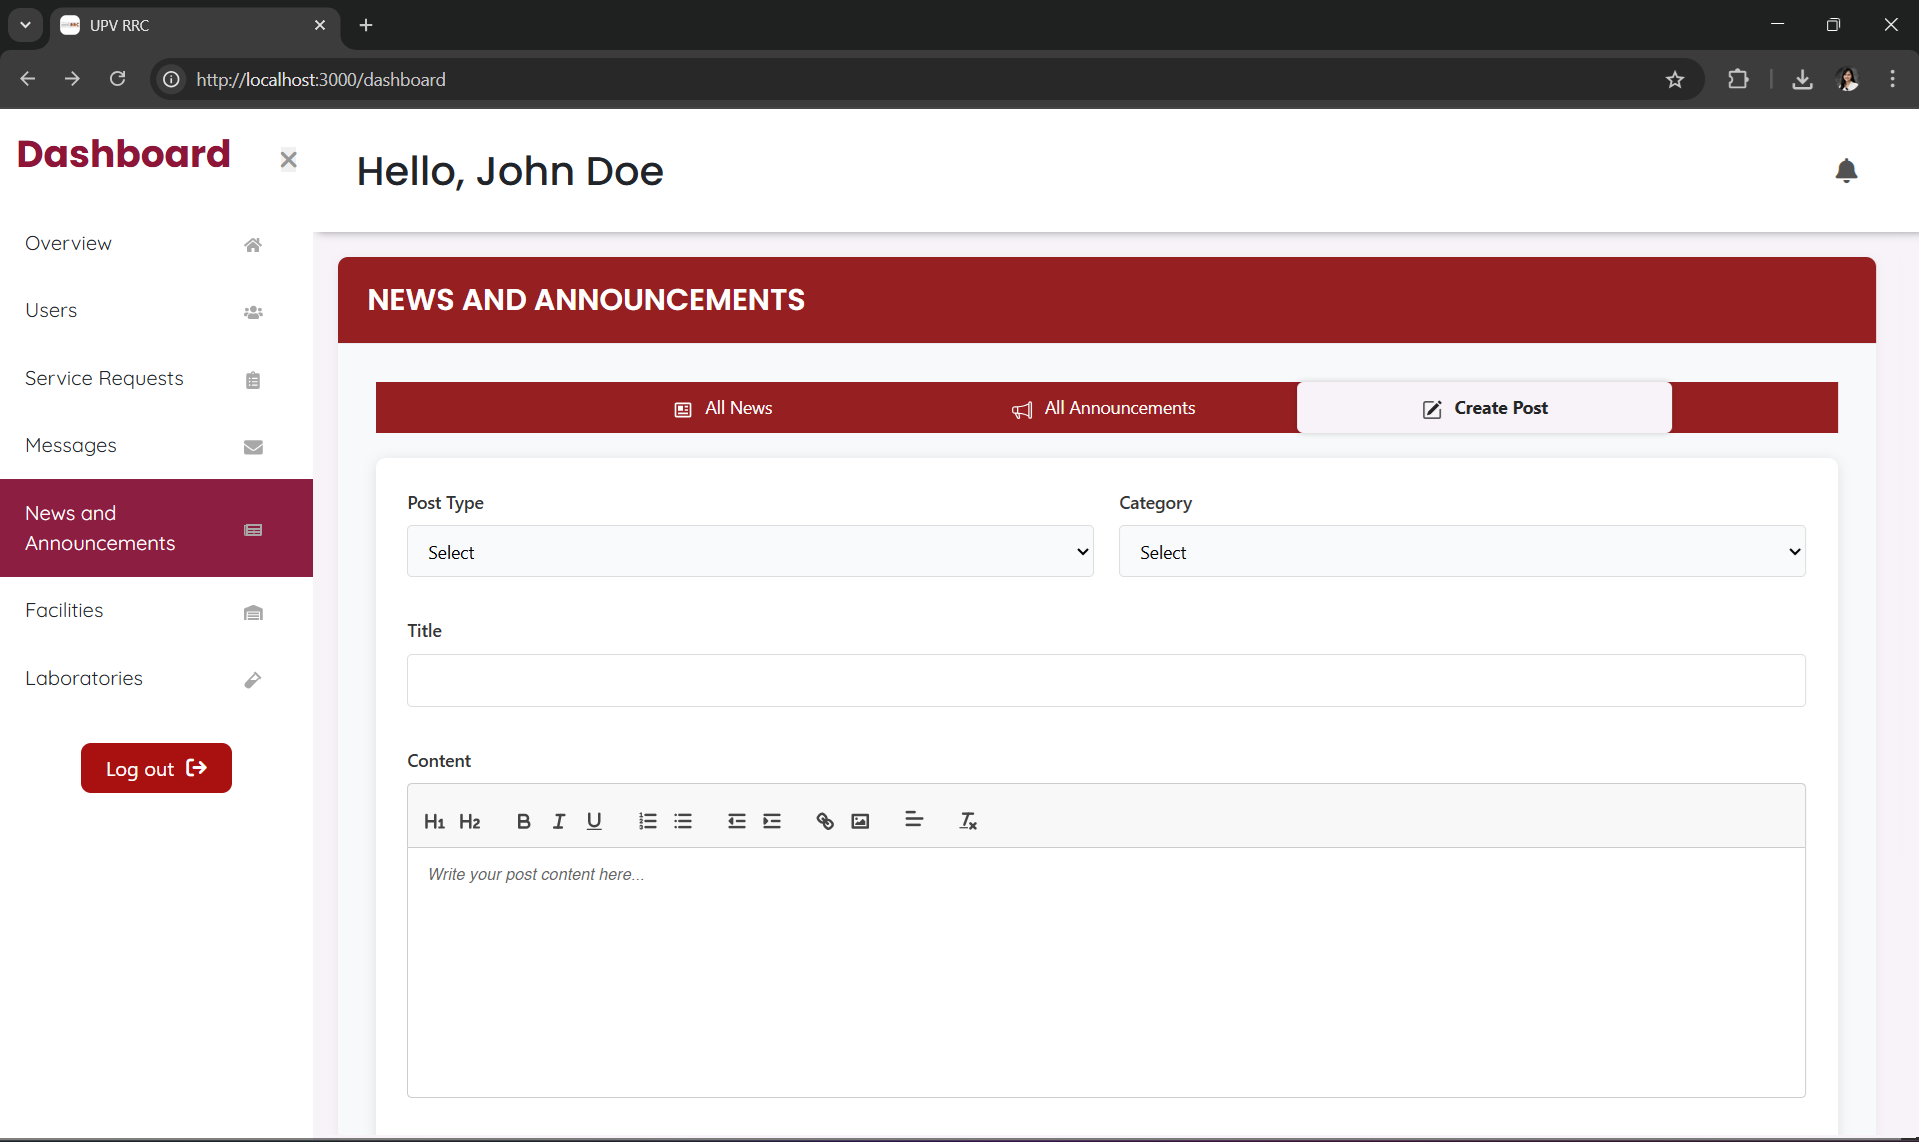
\includegraphics[width=0.8\textwidth]{news_section.png}
    \caption{Interface for creating News and Announcements}
    \label{fig:announcements}
\end{figure}

\newpage

\subsection{Data Management Module}

Data management module is responsible for handling all the data within the system. This includes information of clients, transaction histories, inventory of equipment, and tracking of facility schedules and availability. This modules ensures that accounts are properly maintained while also allowing the staff to easily keep record of everything that is related to the RRC's service requests. It also streamlines the assignment of resources to users, maintains an up-to-date inventory, and provides a comprehensive view of resources, allowing for efficient allocation and tracking. Moreover, it enables staff and clients alike to view real time availability of equipment and facility, further guaranteeing the smooth and efficient flow of  service requests.

\subsection{Chatbot}

The chatbot, named LIRA (Learning, Innovation, and Research Assistant), was successfully integrated into the TUKIB system. It appears as a floating button located at the bottom left corner of each page, allowing users to access assistance at any time.

Upon clicking the button, the chatbot initiates the conversation by presenting a welcome message, as shown in \figref{fig:chatbot_ui}. It then offers a set of predefined options to help users with possible queries. These include inquiries about laboratory services, frequently asked questions, and how to navigate the system. This setup reduces the workload on support staff and improves user satisfaction by providing immediate answers.

\begin{figure}[h]
	\centering
	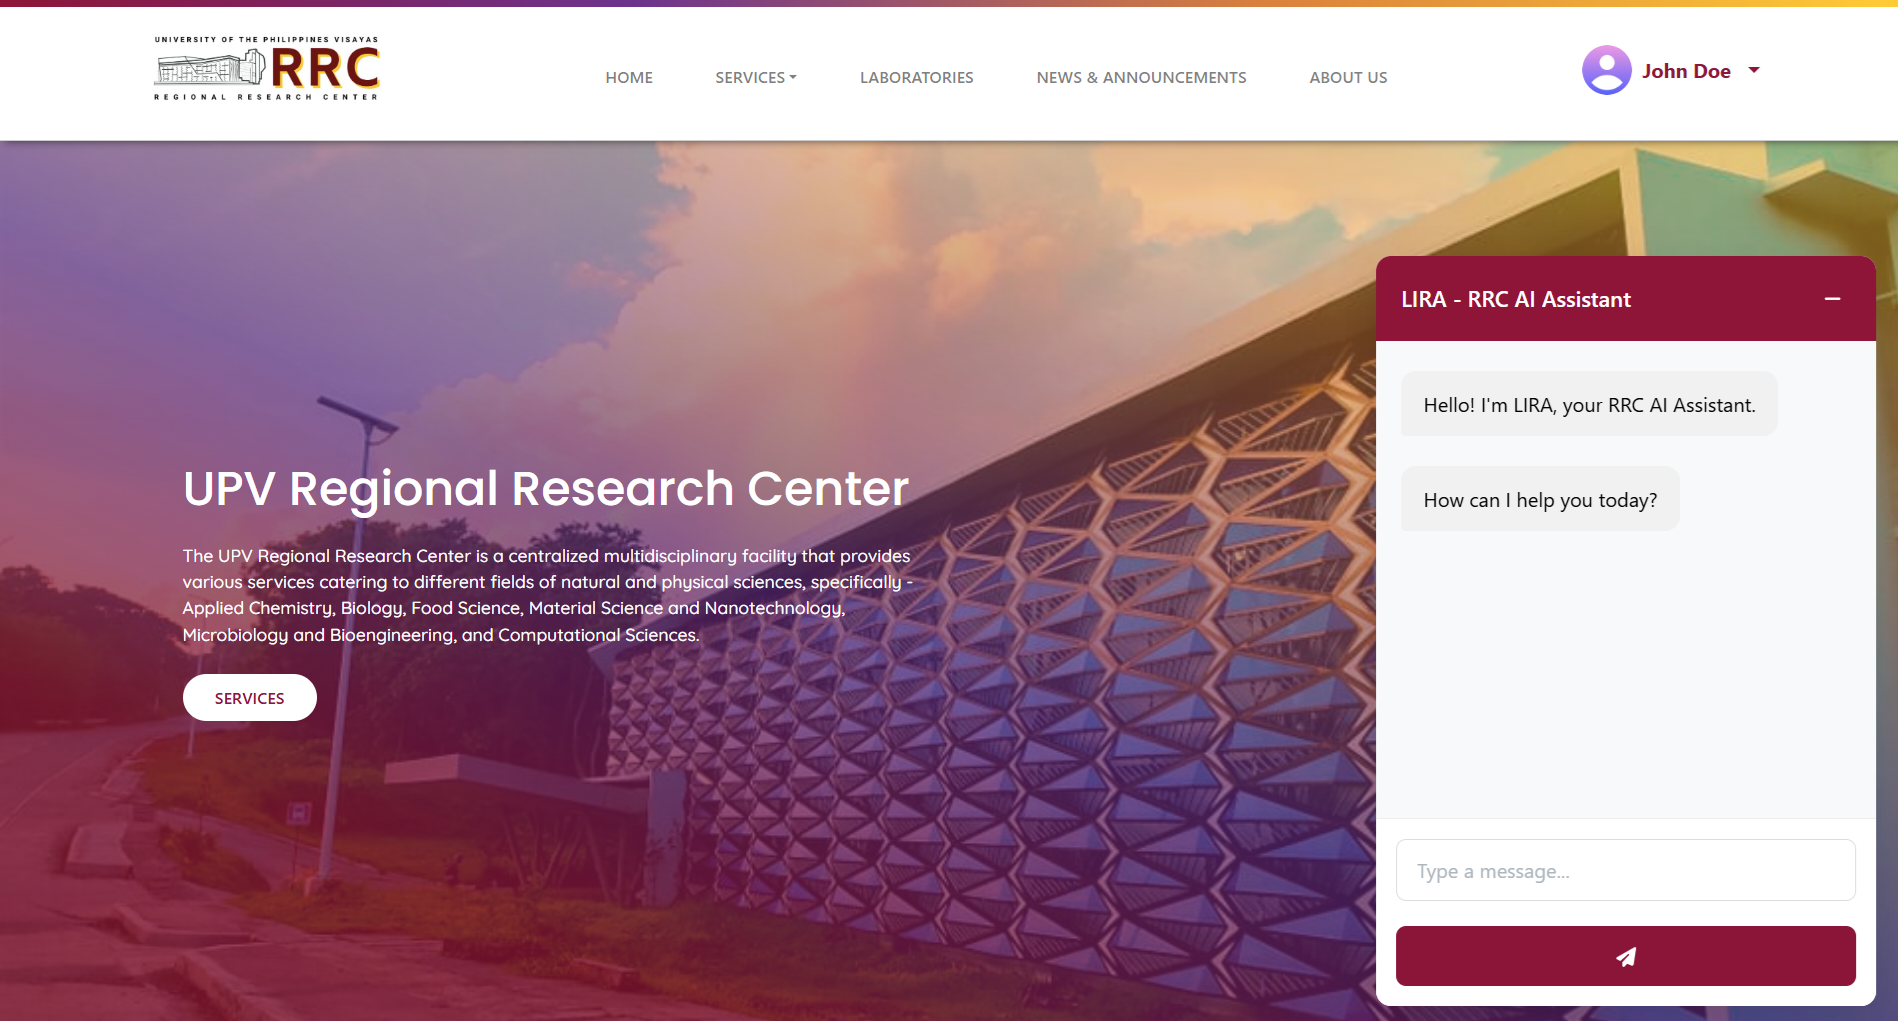
\includegraphics[width=0.8\textwidth]{chatbot_ui.png}
	\caption{Chatbot Interface}
	\label{fig:chatbot_ui}
\end{figure}

\textbf{Functionality}

The chatbot was developed using the Rasa framework, which includes both a Natural Language Understanding (NLU) component and a dialogue management system. It is capable of handling various types of user intents such as greetings, general inquiries, and specific service-related questions. The bot provides options for users to learn about available laboratory services, request procedures, operating hours, and system navigation.

In its current state, LIRA utilizes a set of predefined intents and responses based on a small, curated training dataset relevant to the Regional Research Center (RRC). The chatbot can perform initial consultation with new clients. Once the client's request is deemed feasible, the chatbot proceeds to collect the user’s details and creates the user's account. 

\textbf{Observed Limitations}

While functional, the chatbot currently has several limitations. First, its training data is limited, which restricts the range and depth of questions it can effectively handle. As a result, the bot sometimes fails to provide helpful responses to queries outside its training scope.

Furthermore, during testing, several issues were observed:
\begin{itemize}
    \item The chatbot has difficulty accurately recognizing names of people.
    \item It struggles to interpret numerical data such as dates, phone numbers, and reference codes.
    \item It sometimes returns generic fallback responses to queries that deviate slightly from the expected format.
\end{itemize}

These limitations reduce the chatbot’s ability to handle more complex or varied queries, especially those involving specific personal or transactional information. Despite this, LIRA contributes positively to the overall system by offering an immediate support channel and guiding users toward the appropriate services within TUKIB.

\section{Data Privacy and Security Measures}

Ensuring the privacy and security of user data is a critical component of the TUKIB system. Several technical measures were implemented to protect user credentials, control access, and prepare for potential data loss scenarios.

\subsection{Password Encryption}

In order to ensure the security of user accounts, password hashing was implemented. This ensures that even if the database is compromised, plaintext passwords remain protected. The bcrypt algorithm was used due to its strength and resistance to brute-force attacks. Each password is hashed with a unique salt, which adds randomness and protects against rainbow table attacks.

During user registration, passwords are hashed before being stored in the database. During login, the hashed version of the input password is compared to the stored hash to authenticate users. This approach follows best practices in modern web security and ensures that sensitive credentials are never stored or transmitted in plain text.

\subsection{User Authentication and Authorization}

The system uses secure authentication and authorization mechanisms to manage user access and roles. These mechanisms include:

\begin{itemize}
	\item \textbf{Token-Based Authentication.} JSON Web Tokens (JWTs) are used to authenticate sessions securely. Tokens are issued upon successful login and used to verify user identity in subsequent interactions without exposing sensitive data.
	\item \textbf{Role-Based Access Control (RBAC).} Access to system functionalities is restricted based on user roles. For example, administrators, staff, and clients each have distinct permissions, reducing the risk of unauthorized actions.
	\item \textbf{Login Attempt Restrictions.} To mitigate brute-force attacks, the system enforces login attempt limits. After a specified number of failed login attempts, the account is temporarily locked, and further login attempts are blocked for a cooling-off period.
\end{itemize}

\subsection{Terms and Conditions}

To ensure transparency and user accountability, the TUKIB system includes a Terms and Conditions agreement that users must acknowledge before submitting a service request. This agreement outlines the responsibilities of both the users and the UPV Regional Research Center, including provisions on proper usage of the system, adherence to facility protocols, and consent to data processing.

In the service request form, a checkbox is provided requiring users to confirm that they have read and agreed to the Terms and Conditions before proceeding. A hyperlink to the full Terms and Conditions document is embedded directly in the form text for convenient access. This serves as an initial layer of compliance with the system’s data privacy and security policies.

\begin{figure}[h]
	\centering
	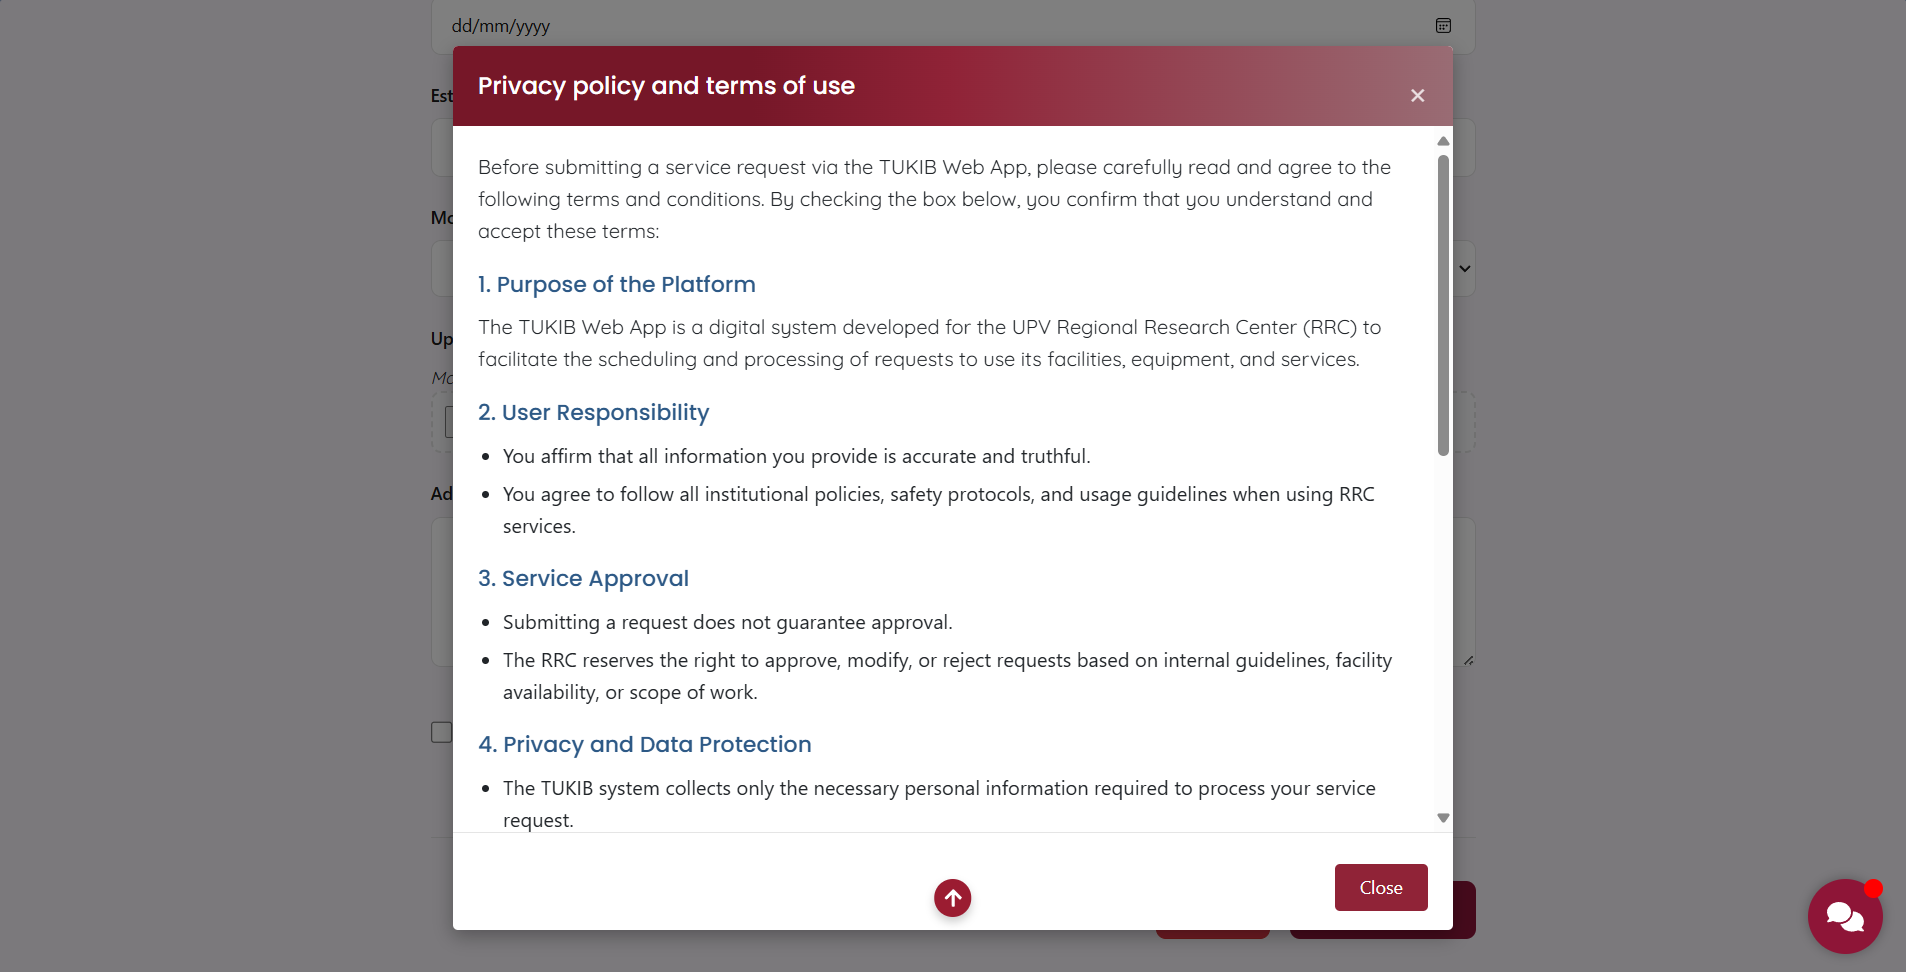
\includegraphics[width=0.8\textwidth]{terms.png}
	\caption{Terms and Conditions}
	\label{fig:terms}
\end{figure}

By requiring agreement to the Terms and Conditions before every service request, the system ensures that users are informed of the scope of their obligations and rights, particularly with regard to the handling of personal and research-related information. This step is crucial in promoting responsible usage and safeguarding sensitive data within the TUKIB platform.

\subsection{Backup and Recovery}

To safeguard against data loss caused by system failures, data breaches, or accidental deletions, automatic data archiving and backup mechanisms were implemented. The system is configured to perform regular backups of critical data, ensuring that recent information can be restored in the event of an incident.

Backups are scheduled at defined intervals and stored securely, following best practices for data integrity and redundancy. These backups can be used to recover the system to a previously stable state, minimizing downtime and preventing permanent data loss. 

\section{Testing and System Evaluation}

System testing was conducted alongside the development process to ensure functionality and usability. This involved thorough manual testing of each feature to identify and resolve bugs during and after implementation. Additionally, an RRC staff was regularly consulted for further information to support informed and context-aware development decisions.

Once the core requirements had been implemented, the complete system underwent an internal review with RRC staff. This initial round of evaluation focused on verifying that the system aligns with RRC's operational needs and identifying specific areas for improvement. The insights of staffs were used to refine certain components of the system, particularly those related to service workflows. 

Subsequently, external testing was conducted with potential end users, mainly students who may serve as future clients of the RRC. These users evaluated the platform based on ease of navigation, intuitiveness, and overall user experience. Feedback was gathered informally through observation and short interviews.

Performance testing was also conducted however, due to resource and technical limitations, the testing was restricted to small-scale scenarios. The focus was on verifying responsiveness and stability during typical operations—such as form submissions, login, chatbot interaction, and navigation— when accessed by one or two users on a local setup. Additionally, cross-browser testing was conducted using popular browsers including Chrome, Firefox, and Edge to ensure consistent functionality and a seamless experience across platforms.

The chatbot LIRA was also tested for its responsiveness and usefulness. While it was generally effective in assisting users with FAQs and service-related inquiries, some limitations were identified. Notably, the chatbot encountered difficulties in accurately handling inputs that included proper names (e.g., names of people), as well as numeric information such as dates and phone numbers. These types of input were sometimes misinterpreted or responded to with irrelevant suggestions. This limitation highlights the need for future enhancements in natural language processing capabilities to allow the chatbot to better understand and handle diverse user inputs.

Overall, feedback from testing indicated a positive reception. RRC staff noted the system’s potential to significantly improve the efficiency of service delivery and resource management. While end users find the system easy to navigate, intuitive, and user-friendly. Performance testing demonstrated that the system operates reliably and responsively under typical usage conditions.

These testing and evaluation phases confirmed the system’s effectiveness in meeting user requirements and provide a strong foundation for future improvements.

\section{Summary of Results}

To summarize the results of the study, the checklist of system requirements, Table \ref{tab:requirements}, was updated to indicate whether each requirement for TUKIB has been implemented. As shown in the Table \ref{tab:summary_results}, all of the system requirements have been successfully accomplished, demonstrating that the core functionalities of TUKIB are in place. Moreover, based on the evaluation and feedback from testing, the final output of this paper was agreed to meet the requirements needed by the users, especially by the RRC staff.

\begin{table}[ht]
	\centering
	\begin{tabular}{|p{10cm}|c|}
		\hline
		\textbf{Requirements/Modules} & \textbf{Accomplished (Y/N)} \\
		\hline
		\multicolumn{2}{|l|}{\textbf{Backend Requirements}} \\
		\hline
		Local Database & Y \\
		Automatic archiving & Y \\
		RESTful API & Y \\
		Role-based access control & Y \\
		Error handling, validation, \& logging & Y \\
		\hline
		\multicolumn{2}{|l|}{\textbf{Privacy Requirements}} \\
		\hline
		User password encryption & Y \\
		Session or token authentication & Y \\
		Restriction of unauthorized access & Y \\
		Log in attempts limit/Brute-force protection & Y \\
		\hline
		\multicolumn{2}{|l|}{\textbf{User Interface Requirements}} \\
		\hline
		Client interface & Y \\
		Admin Staff interface & Y \\
		University Researcher interface & Y \\
		TECD Staff interface & Y \\
		Director interface & Y \\
		\hline
		\multicolumn{2}{|l|}{\textbf{Functional Requirements}} \\
		\hline
		User registration and authentication & Y \\
		Request tracking and management & Y \\
		Feedback mechanism & Y \\
		Notification system & Y \\
		Calendar system & Y \\
		Chatbot for FAQs and initial consultation & Y \\
		End-to-end flow of service request process & Y \\
		\hline
		\multicolumn{2}{|l|}{\textbf{UI/UX Design Requirements}} \\
		\hline
		Responsive design & Y \\
		User-friendly navigation & Y \\
		Feedback/confirmation messages & Y \\
		\hline
	\end{tabular}
	\caption{System Requirements Checklist Result}
	\label{tab:summary_results}
\end{table}